\documentclass[hyperref={pdfpagelabels=false},compress]{beamer} 
\let\Tiny=\tiny
\usepackage{lmodern}% http://ctan.org/pkg/lm
\mode<presentation>
{\usetheme{Berlin} \setbeamercovered{transparent}}
\usetheme{Ilmenau}
\usepackage{lipsum}
\setbeamerfont*{section in head/foot}{size=\tiny}
\setbeamerfont*{subsection in head/foot}{size=\large}

\newlength\SubHt
\settoheight\SubHt{\usebeamerfont{subsection in head/foot}S}
\newlength\SubDh
\settodepth\SubDh{\usebeamerfont{subsection in head/foot}g}

\makeatletter
\setbeamertemplate{headline}
{%
  \begin{beamercolorbox}[colsep=1.5pt]{upper separation line head}
  \end{beamercolorbox}
  \begin{beamercolorbox}{section in head/foot}
    \vskip2pt\insertnavigation{\paperwidth}\vskip2pt
  \end{beamercolorbox}%
  \ifbeamer@theme@subsection%
    \begin{beamercolorbox}[colsep=1.5pt]{middle separation line head}
    \end{beamercolorbox}
    \begin{beamercolorbox}[ht=1.5\SubHt,dp=1.5\SubDh,%defaults: ht=2.5ex,  dp=1.125ex
      leftskip=.3cm,rightskip=.3cm plus1fil]{subsection in head/foot}
      \usebeamerfont{subsection in head/foot}\insertsubsectionhead
    \end{beamercolorbox}%
  \fi%
  \begin{beamercolorbox}[colsep=1.5pt]{lower separation line head}
  \end{beamercolorbox}
}
\makeatother

\usetheme{Ilmenau}
\usepackage{amsmath} 
\usepackage{amssymb} 
\usepackage{graphicx}
\usepackage{subfigure}
\usepackage{listings}
\usepackage{xcolor}
\usepackage{tabularx,booktabs}

\usepackage[utf8]{inputenc}
\usepackage{hyperref}

\usepackage[english]{babel}

\setbeamerfont*{subsection in head/foot}{size=\large}
\newcolumntype{C}[1]{>{\centering\arraybackslash}p{#1}}

% Default fixed font does not support bold face
\DeclareFixedFont{\ttb}{T1}{txtt}{bx}{n}{12} % for bold
\DeclareFixedFont{\ttm}{T1}{txtt}{m}{n}{12}  % for normal

\graphicspath{ {pdf/} }

% Custom colors
\usepackage{color}

\lstset{classoffset=0,
morekeywords={mkdir, cd, alias,ln,df, awk,ls,git,wget,cat, perl,echo, export,python,next,if,fi,then, for,my,return,tr,ps,do,done, top,substr,ord,length,qstat},
keywordstyle=\color{blue},classoffset=1,
morekeywords={sub,exit,function,def},keywordstyle=\color{red},classoffset=0,
morecomment=[l][\color{teal}]{\#},
basicstyle=\ttfamily\scriptsize,
backgroundcolor=\color[rgb]{0.95,0.95,0.95},
breaklines=true}

\begin{document}
%%-------------------------------------------------
    \title{Comparison of Tophat and Hisat mapping results for real data.}
    \author{Boqiang Hu}
    \institute{ Laboratory of Stem Cells and Epigenetics, BIOPIC, Peking University }
    \date{\today}
    \begin{frame}
    	 \titlepage
    \end{frame}
%%-------------------------------------------------

\section{The work flow of Tophat}

\subsection{ Before running: Two important parameters. }
\begin{frame}[c,fragile]
	\scriptsize{
		\begin{block}{ Transcriptome or Genome level? \alert{ -G } }
			\begin{itemize}
				\item If -G tag were used, reads would be first mapped to transcriptome rather than genome at the very beginning, then those unmapped reads would be used to find genome-reads, new-transcripts, even fusions(optional). \\ \pause
				\item As I used to analyse human or mouse data, whose transcriptome were well annotated, so here, -G tag were highly recommanded. \pause
			\end{itemize}
		\end{block}
		\begin{block}{ Keep the tmp files during mapping. \alert{ --keep-tmp } }
			\begin{itemize}
				\item	If you simply want to calculate FPKM, find different expressed genes or so on, keep tmp file would be simply a waste of disk-space.   \\ \pause
				\item But, if you want to search for \alert{fusion gene} or \alert{circular RNAs}, or even to get a \alert{precise result for lincRNA}(Long intergenic noncoding RNA), --keep-tmp tag were recommended while running tophat, which could tell you how tophat pipeline works, and how each tool was used in the whole pipeline.
			\end{itemize}
		\end{block}
	}
\end{frame}

\subsection{ Step1. Preparing for transcriptome reference.}
\begin{frame}[c,fragile]

	\begin{block}{ Prepare the junctions. }
		\begin{lstlisting}
$tophat_bin_dir/gtf_juncs    \
   $gtf_dir/genes.gtf        \
  >$root_dir/genes.juncs
		\end{lstlisting}
	\end{block}

	\begin{block}{ Prepare the transcriptome bowtie-fasta. }
		\begin{lstlisting}
$tophat_bin_dir/gtf_to_fasta  \
   $gtf_dir/genes.gtf         \
   $genome $root_dir/genes.fa
	
bowtie2-build 						\
   $root_dir/genes.fa         \
   $root_dir/genes
		\end{lstlisting}
	\end{block}
\end{frame}

	
	
\subsection{ Step2. Preparing for input reads.}
\begin{frame}[c,fragile]


	\begin{block}{ scripts }
		\begin{lstlisting}[basicstyle=\tiny]
# Convert fq to a bam without mapping. Position information were null in this bam and illumina read-id would be convert to a new id (from 1 to total-input reads). (using default parameter)
### input:  *.1.clean.fq.gz,     *.2.clean.fq.gz
### output: left_kept_reads.bam	right_kept_reads.bam

$bin_dir/prep_reads                                        \
    --gtf-annotations $gtf_dir/genes.gtf                   \
    --gtf-juncs $root_dir/genes.juncs 	                    \
    --aux-outfile=$root_dir/../prep_reads.info             \
    --index-outfile=$root_dir/%side%_kept_reads.bam.index  \
    --sam-header=$root_dir/genome_genome.bwt.samheader.sam \
    --outfile=$root_dir/%side%_kept_reads.bam              \
    Input.1.fq.gz Input.2.clean.fq.gz
		\end{lstlisting}
	\end{block}
\end{frame}



\subsection{ Step3. Mapping to transcriptome.}
\begin{frame}[c,fragile]
	\begin{block}{ Why not using BWA directly? }
		\begin{itemize}
			\item The different between BWA and tophat is that BWA only do this step, and Tophat did a lot more after this step, and simply using BWA is pair-end mapping.\\ \pause
			\item Tophat use \alert{single-end} mapping then merge the SE result.
		\end{itemize}
	\end{block}
\end{frame}
\begin{frame}[c,fragile]
	\begin{block}{ The \alert{transcriptome-mapped-reads} could be detected via: }
		\begin{lstlisting}[basicstyle=\tiny]
### input:  left_kept_reads.bam              (right side is the same)
### output: left_kept_reads.m2g_um.bam       (not mapped to transcriptome)
###         left_kept_reads.m2g.bam          (tran-mapped result for genome location)
### tmp:left_kept_reads.test_step1.bam	(tmp file for bowtie. bowtie result for all prepared reads).
###     left_kept_reads.test_step2.bam	(tran-mapped result for transcriptome location)

$bin_dir/bam2fastx --all $root_dir/left_kept_reads.bam|    \
bowtie2 -x $root_dir/genes -                            |  \
$bin_dir/fix_map_ordering                                  \
    --sam-header $root_dir/genes.bwt.samheader.sam         \
    - -                                                    \
    $root_dir/left_kept_reads.m2g_um.bam                |  \
$bin_dir/map2gtf                                           \
    --sam-header $root_dir/genome_genome.bwt.samheader.sam \
    $root_dir/genes.fa.tlst -                              \
    $root_dir/left_kept_reads.m2g.bam
		\end{lstlisting}
	\end{block}
\end{frame}






\subsection{ Step4. Mapping to genome.} 
\begin{frame}[c,fragile]
	\begin{block}{ How to deal with \alert{transcriptome-unmapped} reads? }
		\begin{itemize}
			\item In BWA-protocal of our lab does, the transcriptome-unmapped reads were discard or then mapped to ensemble, noncode, and then to genome, finally for novo-lincRNA assembling, just as nsmb.2660 did.\\ \pause
			\item However, as ensemble and noncode  are all annotated based on genome, we can directly \alert{map those reads to genome}, which would get more mapped reads because there might be reads of novo-lincRNA which were not recorded in ensemble, and cannot map to genome because of there were \alert{junction reads in this novo-lincRNA}.
		\end{itemize}
	\end{block}
\end{frame}
\begin{frame}[c,fragile]
	\begin{block}{ The \alert{genome-mapped-reads} could be detected via: }
		\begin{lstlisting}[basicstyle=\tiny]
### input:  left_kept_reads.m2g_um.bam              (right side is the same)
### output: left_kept_reads.m2g_um.mapped.bam       (tran NO genome YES)
###         left_kept_reads.m2g_um.unmapped.bam     (tran NO genome NO )
### tmp:    left_kept_reads.m2g_um_seg1.fq.z        (divide unmapped 101bp into 4 parts fq )
###         left_kept_reads.m2g_um_seg2.fq.z
###         left_kept_reads.m2g_um_seg3.fq.z
###         left_kept_reads.m2g_um_seg4.fq.z

$bin_dir/bam2fastx                                 \
    --all $root_dir/left_kept_reads.bam          | \
bowtie2                                            \
    -x $genome -                                 | \
    $bin_dir/fix_map_ordering                      \
    --sam-header $root_dir/genes.bwt.samheader.sam \
    - -                                            \
    $root_dir/left_kept_reads.m2g_um.mapped.bam    \
    $root_dir/left_kept_reads.m2g_um.unmapped.bam
		\end{lstlisting}
	\end{block}
\end{frame}


\subsection{ Step5. Mapping to genome with junctions.} 
\begin{frame}[c,fragile]
	\begin{block}{ How to deal with genome-mapped reads with junctions? }
		\begin{itemize}
			\item Only this step could not detect those reads with junctions in novo-lincRNA or a newly detected isoform for a known gene.\\ \pause
			\item So here the reads were split into (readlen/25) \alert{segments}, (e.g, 4 parts for 101bp reads) then map to genome:
		\end{itemize}
	\end{block}
\end{frame}
\begin{frame}[c,fragile]
	\begin{block}{ The \alert{junctional genome-mapped-reads} could be detected via: }
		\begin{lstlisting}[basicstyle=\tiny]
### input:  left_kept_reads.m2g_um_seg1.fq.z          
     (right side, 2 3 4 are the same)
### output: left_kept_reads.m2g_um_seg1.to_spliced.bam
     (tran NO genome NO, first25bp genome YES)

gzip -cd< $root_dir/left_kept_reads.m2g_um_seg1.fq.z | \
bowtie2 -k 41 -N 1 -L 20 -p 8 --sam-no-hd              \
    -x $bin_dir/segment_juncs -                      | \
$bin_dir/fix_map_ordering                              \
    --index-outfile $root_dir/left_kept_reads.m2g_um_seg1.to_spliced.bam.index \
    --sam-header    $root_dir/segment_juncs.bwt.samheader.sam \
    - $root_dir/left_kept_reads.m2g_um_seg1.to_spliced.bam
		\end{lstlisting}
	\end{block}
\end{frame}
\begin{frame}[c,fragile]
	\begin{block}{ The \alert{junctional genome-mapped-reads} could be detected via: }
		\begin{lstlisting}[basicstyle=\tiny]
$bin/segment_juncs           #detect junctions
$bin/juncs_db                #build fasta file for junctions
$bin/long_spanning_reads     #merge the mapping information of the 4-parts mapping results.
### one example in left_kept_reads.m2g_um.candidates.bam:
#seg1
662|0:0:4   0  chr2    110423264  0   25M          ...
662|0:0:4   0  chr20   60962952   0   18M1I6M      ...

#seg2
662|25:1:4  0   chr20  60963371   32  25M          ...
662|25:1:4  16  chr4   16257966   32  25M          ...

#seg3
662|50:2:4  0   chr20  60963396   255 25M          ...

#seg4
662|75:3:4  0   chr20  60963421   255 26M          ...

#candidates:
662         0   chr20  60962952   255 19M394N82M   ...
		\end{lstlisting}
	\end{block}
\end{frame}


\subsection{ After mapping: How to make good use of the tmp files? } 
\begin{frame}[c,fragile]
	\begin{block}{ Classify of reads in bam files: }
		\begin{lstlisting}[basicstyle=\tiny]
   transcriptome-mapped          Left      accepted.bam
   genome-mapped                 Left      accepted.bam
   genome-mapped-junction-reads  Left      accepted.bam
   transcriptome-mapped          Right     accepted.bam
   genome-mapped                 Right     accepted.bam
   genome-mapped-junction-reads  Right     accepted.bam
   unmapped                      OneSide   accepted.bam
   unmapped                      TwoSides  unmapped.bam
		\end{lstlisting}
	\end{block}
\end{frame}

\begin{frame}[c,fragile]
	\begin{block}{ In details: }
		\begin{lstlisting}[basicstyle=\tiny]
   L-transcriptome-mapped     left_kept_reads.m2g.bam               
   L-genome-mapped            left_kept_reads.m2g_um.mapped.bam     
   L-genome-mapped-junc-reads left_kept_reads.m2g_um.candidates.bam 
   R-transcriptome-mapped     right_kept_reads.m2g.bam              
   R-genome-mapped            right_kept_reads.m2g_um.mapped.bam
   R-genome-mapped-junc-reads right_kept_reads.m2g_um.candidates.bam 
   L-unmapped                 left.............m2g_um.unmapped.bam
                                               m2g_um.candidates.bam
   R-unmapped                 right............m2g_um.unmapped.bam
                                               m2g_um.candidates.bam

		\end{lstlisting}
		For fusion data:
		\begin{itemize}
			\item PE1 and PE2 in L/R transcriptome-mapped file, but distally. \pause
			\item PE1 and PE2.seg1, seg2  in L-transcriptome-mapped, \\PE2.seg4 in R-transcriptome-mapped distally. \\PE2.seg3 were fusion reads.
		\end{itemize}
	\end{block}
\end{frame}

\begin{frame}[c,fragile]
	\begin{block}{ How to deal with \alert{transcriptome-unmapped} reads? }
		\begin{itemize}
			\item One possible method for detecting circular-RNA using Tophat. See https://github.com/YangLab/CIRCexplorer \\ \pause
			\item For pair-end data, one possible method: https://github.com/hubqoaing/TanglabCircularRNAPipeline
		\end{itemize}
	\end{block}
\end{frame}

\section{1.Running comparison analysis frame-work. } 
\subsection{1. Build the analysis dictionary.}
\begin{frame}[c,fragile]
	\begin{block}{ First build the root\_dir. }
		\begin{lstlisting}
mkdir $root_dir && cd $root_dir
		\end{lstlisting}
	\end{block}
	\pause
	\begin{block}{ Download the scripts. Python required.}
		All code for analysis were in my github.
		\begin{lstlisting}
git clone https://github.com/hubqoaing/RNA_Comp
cd RNA_Comp
		\end{lstlisting}
	\end{block}
\end{frame}

\subsection{2. Download GSM981249 sra data.}
\begin{frame}[c,fragile]
	\begin{block}{ Download Raw data. }
		\begin{lstlisting}
mkdir -p 00.fastq/SRR534301
cd       00.fastq/SRR534301
wget ftp://ftp-trace.ncbi.nlm.nih.gov/sra/sra-instant/reads/ByExp/sra/SRX/SRX174/SRX174318/SRR534301/SRR534301.sra
		\end{lstlisting}
	\end{block}
\end{frame}

\subsection{3. Preparing the input files.}
\begin{frame}[c,fragile]

	\begin{block}{ Input reference. }
Detailed information for input files could be reached in:
\url{https://github.com/hubqoaing/RNA} \\
To run Hisat, it was required to build a Hisat-index for the fasta reference.
		\begin{lstlisting}
hisat-build hg19_ERCC92_RGC.fa hg19_ERCC92_RGC.hisat
		\end{lstlisting}
	\end{block}
	\pause
	\begin{block}{ sample list. }
		\begin{lstlisting}[basicstyle=\tiny]
$ cat sample_GSM981249.xls
sample_name		sample_brief_name		stage			sample_group	ERCC_times	RFP_polyA	GFP_polyA	CRE_polyA	data_type	rename
SRR534301		test_SRR534301			RealData		RNA            0.0    		0.0    		0.0		   0.0		 	PE          SRR534301
		\end{lstlisting}
	\end{block}

\end{frame}

\subsection{4. Generate all scripts for mapping pipeline.}
\begin{frame}[c,fragile]

	\begin{block}{ Debug mode. Generate scripts but do not run it. }
A python script could be written with the guidance of the README.md file. \\
Run the following scripts to generate all shell scripts. Then check it by running step by step.
		\begin{lstlisting}[basicstyle=\tiny]
python run_mRNA.py                               \
   --bt_index_base  hg19_ERCC92_RGC              \
   --genome_gtf     hg19_ERCC92_RGC_refGene.gtf  \
   --intragenic_bed region.Intragenic.bed        \
   --refGene_hg19   ref.sort.txt                 \
   --ercc_info      ercc.info.xls                \
   --rmsk_gtf       region.Intragenic.filter.bed \
   --genome_gtf_with_lncRNA  Early_Embroy_LncRNA_Pool.ERCC_RGCPolyA.sort.gtf  \
   sample_GSM981249.xls
		\end{lstlisting}
	\end{block}
\end{frame}


\subsection{5. Scripts for mapping.}
\begin{frame}[c,fragile]
	\begin{block}{ 1. Tophat mapping to transcriptome first. }
		\begin{lstlisting}[basicstyle=\tiny]
$tophat_py                                       \
   -p 8 -G $gtf_file                             \
   --library-type fr-unstranded                  \    
   --phred64-quals                               \
   -o $tophat_dir/$brief_name                    \
   $genome                                       \
   $fq_dir/$samp_name/$samp_name.1.fq.gz         \
   $fq_dir/$samp_name/$samp_name.2.fq.gz

$samtools sort                                   \
   -n $tophat_dir/$brief_name/accepted_hits.bam  \
	   $tophat_dir/$brief_name/accepted_hits.order
		\end{lstlisting}
	\end{block}
\end{frame}

\begin{frame}[c,fragile]
	\begin{block}{ 2. Tophat using the mannual in HISAT article. }
		\begin{lstlisting}[basicstyle=\tiny]
$tophat_py                                        \
   -p 8                                           \
   --read-edit-dist 3                             \
   --read-realign-edit-dist 3                     \
   --no-sort-bam                                  \
   --phred64-quals                                \
   -o $tophat_dir/$brief_name                     \
   $genome                                        \
   $fq_dir/$samp_name/$samp_name.1.fq.gz          \
   $fq_dir/$samp_name/$samp_name.2.fq.gz

$samtools sort                                    \
   -n $tophat_dir/$brief_name/accepted_hits.bam   \
	   $tophat_dir/$brief_name/accepted_hits.order
		\end{lstlisting}
	\end{block}
\end{frame}

\begin{frame}[c,fragile]
	\begin{block}{ 3. Hisat mapping to transcriptome first. }
		\begin{lstlisting}[basicstyle=\tiny]
$hisat         -p 8 -x $genome --phred64          \
   -1 $fq_dir/$samp_name/$samp_name.1.fq.gz       \
   -2 $fq_dir/$samp_name/$samp_name.2.fq.gz       \
   -S /dev/stdout                                 \
   --known-splicesite-infile $splice_file         \
   2>$hisat_dir/$brief_name/log                  |\
awk '{if($1 ~ /^@/) print $0; else{ for(i=1;i<=NF;i++) if($i!~/^XS/) printf("%s\\t",$i);else XS0=$i;  XS1=((and($2, 0x10) && and($2, 0x40)) || (and($2,0x80) && !and($2,0x10)))?"XS:A:+":"XS:A:-"; print XS1 } }' | \
awk '{if(length($10)==length($11)){print $0}}'   |\
$samtools_exe view                                \
   -Sb -q 1 -                                     \
  >$hisat_dir/$brief_name/accepted_hits.raw.bam &&\
$samtools_exe sort                                \
   -m 2000000000                                  \
   $hisat_dir/$brief_name/accepted_hits.raw.bam   \
   $hisat_dir/$brief_name/accepted_hits		
		\end{lstlisting}
	\end{block}
\end{frame}

\begin{frame}[c,fragile]
	\begin{block}{ 4. Hisat x2 using the mannual in HISAT article. }
		\begin{lstlisting}[basicstyle=\tiny]
$hisat         -p 8 -x $genome --phred64          \
   -1 $fq_dir/$samp_name/$samp_name.1.fq.gz       \
   -2 $fq_dir/$samp_name/$samp_name.2.fq.gz       \
   -S /dev/null                                   \
   --novel-splicesite-outfile $splice_file        \
   2>$hisat_dir/$brief_name/log                && \
$hisat         -p 8 -x $genome --phred64          \
   -1 $fq_dir/$samp_name/$samp_name.1.fq.gz       \
   -2 $fq_dir/$samp_name/$samp_name.2.fq.gz       \
   -S /dev/stdout                                 \
   --novel-splicesite-infile  $splice_file        \
   2>$hisat_dir/$brief_name/log.2                |\
awk '{if($1 ~ /^@/) print $0; else{ for(i=1;i<=NF;i++) if($i!~/^XS/) printf("%s\\t",$i);else XS0=$i;  XS1=((and($2, 0x10) && and($2, 0x40)) || (and($2,0x80) && !and($2,0x10)))?"XS:A:+":"XS:A:-"; print XS1 } }' | \
awk '{if(length($10)==length($11)){print $0}}'   |\
$samtools_exe view                                \
   -Sb -q 1 -                                     \
   >$hisat_dir/$brief_name/accepted_hits.raw.bam &&\
$samtools_exe sort                                \
  -m 2000000000                                   \
  $hisat_dir/$brief_name/accepted_hits.raw.bam    \
  $hisat_dir/$brief_name/accepted_hits
		\end{lstlisting}
	\end{block}
\end{frame}



\subsection{6. Running all scripts when no bug were detected.}
\begin{frame}[c,fragile]

	\begin{block}{ Running scripts in pipeline. }
Removing the comments in \alert{running\_multi} function of \alert{module\_running\_jobs.py}. Run the code above again so that all scriptes could be run one by one.
		\begin{lstlisting}[basicstyle=\tiny]
python run_comp.py                                \
   --bt_index_base  hg19_ERCC92_RGC               \
   --genome_gtf     hg19_ERCC92_RGC_refGene.gtf   \
   --intragenic_bed region.Intragenic.bed         \
   --refGene_hg19   ref.sort.txt                  \
   --ercc_info      ercc.info.xls                 \
   --rmsk_gtf       region.Intragenic.filter.bed  \
   --genome_gtf_with_lncRNA  Early_Embroy_LncRNA_Pool.ERCC_RGCPolyA.sort.gtf  \
   sample_GSM981249.comp.xls
		\end{lstlisting}
	\end{block}
\end{frame}




\subsection{.}
\section{2. Comparing the Read Data. } 

\subsection{1. What concern about are...}
\begin{frame}[c,fragile]
	\begin{block}{ Difference in regions: }
		\begin{itemize}
			\item Gene regions.
			\begin{itemize}
				\item Difference FPKM (cufflinks)? \\
				\item Difference Read Counts (Hiseq)? \\
			\end{itemize}
			\item Repeat regions.
			\begin{itemize}
				\item Difference FPKM (cufflinks)? \\
				\item Difference Read Counts (Hiseq)? \\
			\end{itemize}
		\end{itemize}
	\end{block}
\end{frame}


\subsection{2.Reads mapped to gene-region.}

\begin{frame}[c,fragile]
	\frametitle{ For refseq genes, TT $>$ HT $\approx$ HM $>$ TM. }
		\tiny{
			\begin{table}
			\centering
			\begin{tabular}{  C{0.4cm}  C{1.3cm}  C{1.3cm}  C{1.3cm}  C{1.3cm} C{1.0cm} C{0.75cm} C{0.75cm} }
			\hline\noalign{\smallskip}
			Samp & Pre & Aln & Known & Rfseq & Non4 & Nsmb & Neo \\
			\noalign{\smallskip}\hline\noalign{\smallskip}			
			TT &	217,499K & 181,322K & 172,295K & 170,471K & 1,816K & 7604 & 34486	 \\
			TM &	217,499K & 177,886K & 157,031K & 153,429K & 3,593K & 8000 & 214952  \\
			HT &	217,499K & 195,486K & 165,746K & 163,356K & 2,382K & 8236 & 65284	 \\
			HM &	217,499K & 195,455K & 165,575K & 163,186K & 2,380K & 8238 & 65506	 \\
			\noalign{\smallskip}\hline  		\\
			\end{tabular}
			\end{table}
		}
	
\end{frame}


\begin{frame}[c,fragile]
	\frametitle{ Result calculated by cuffquant-cuffnorm. }
	\begin{block}{ FPKM for genes. }
			\begin{table}
			\centering	
			\begin{tabular}{C{4cm}  C{4cm}}     
				Transcripts in genome		& ERCC spike-ins 	\\
				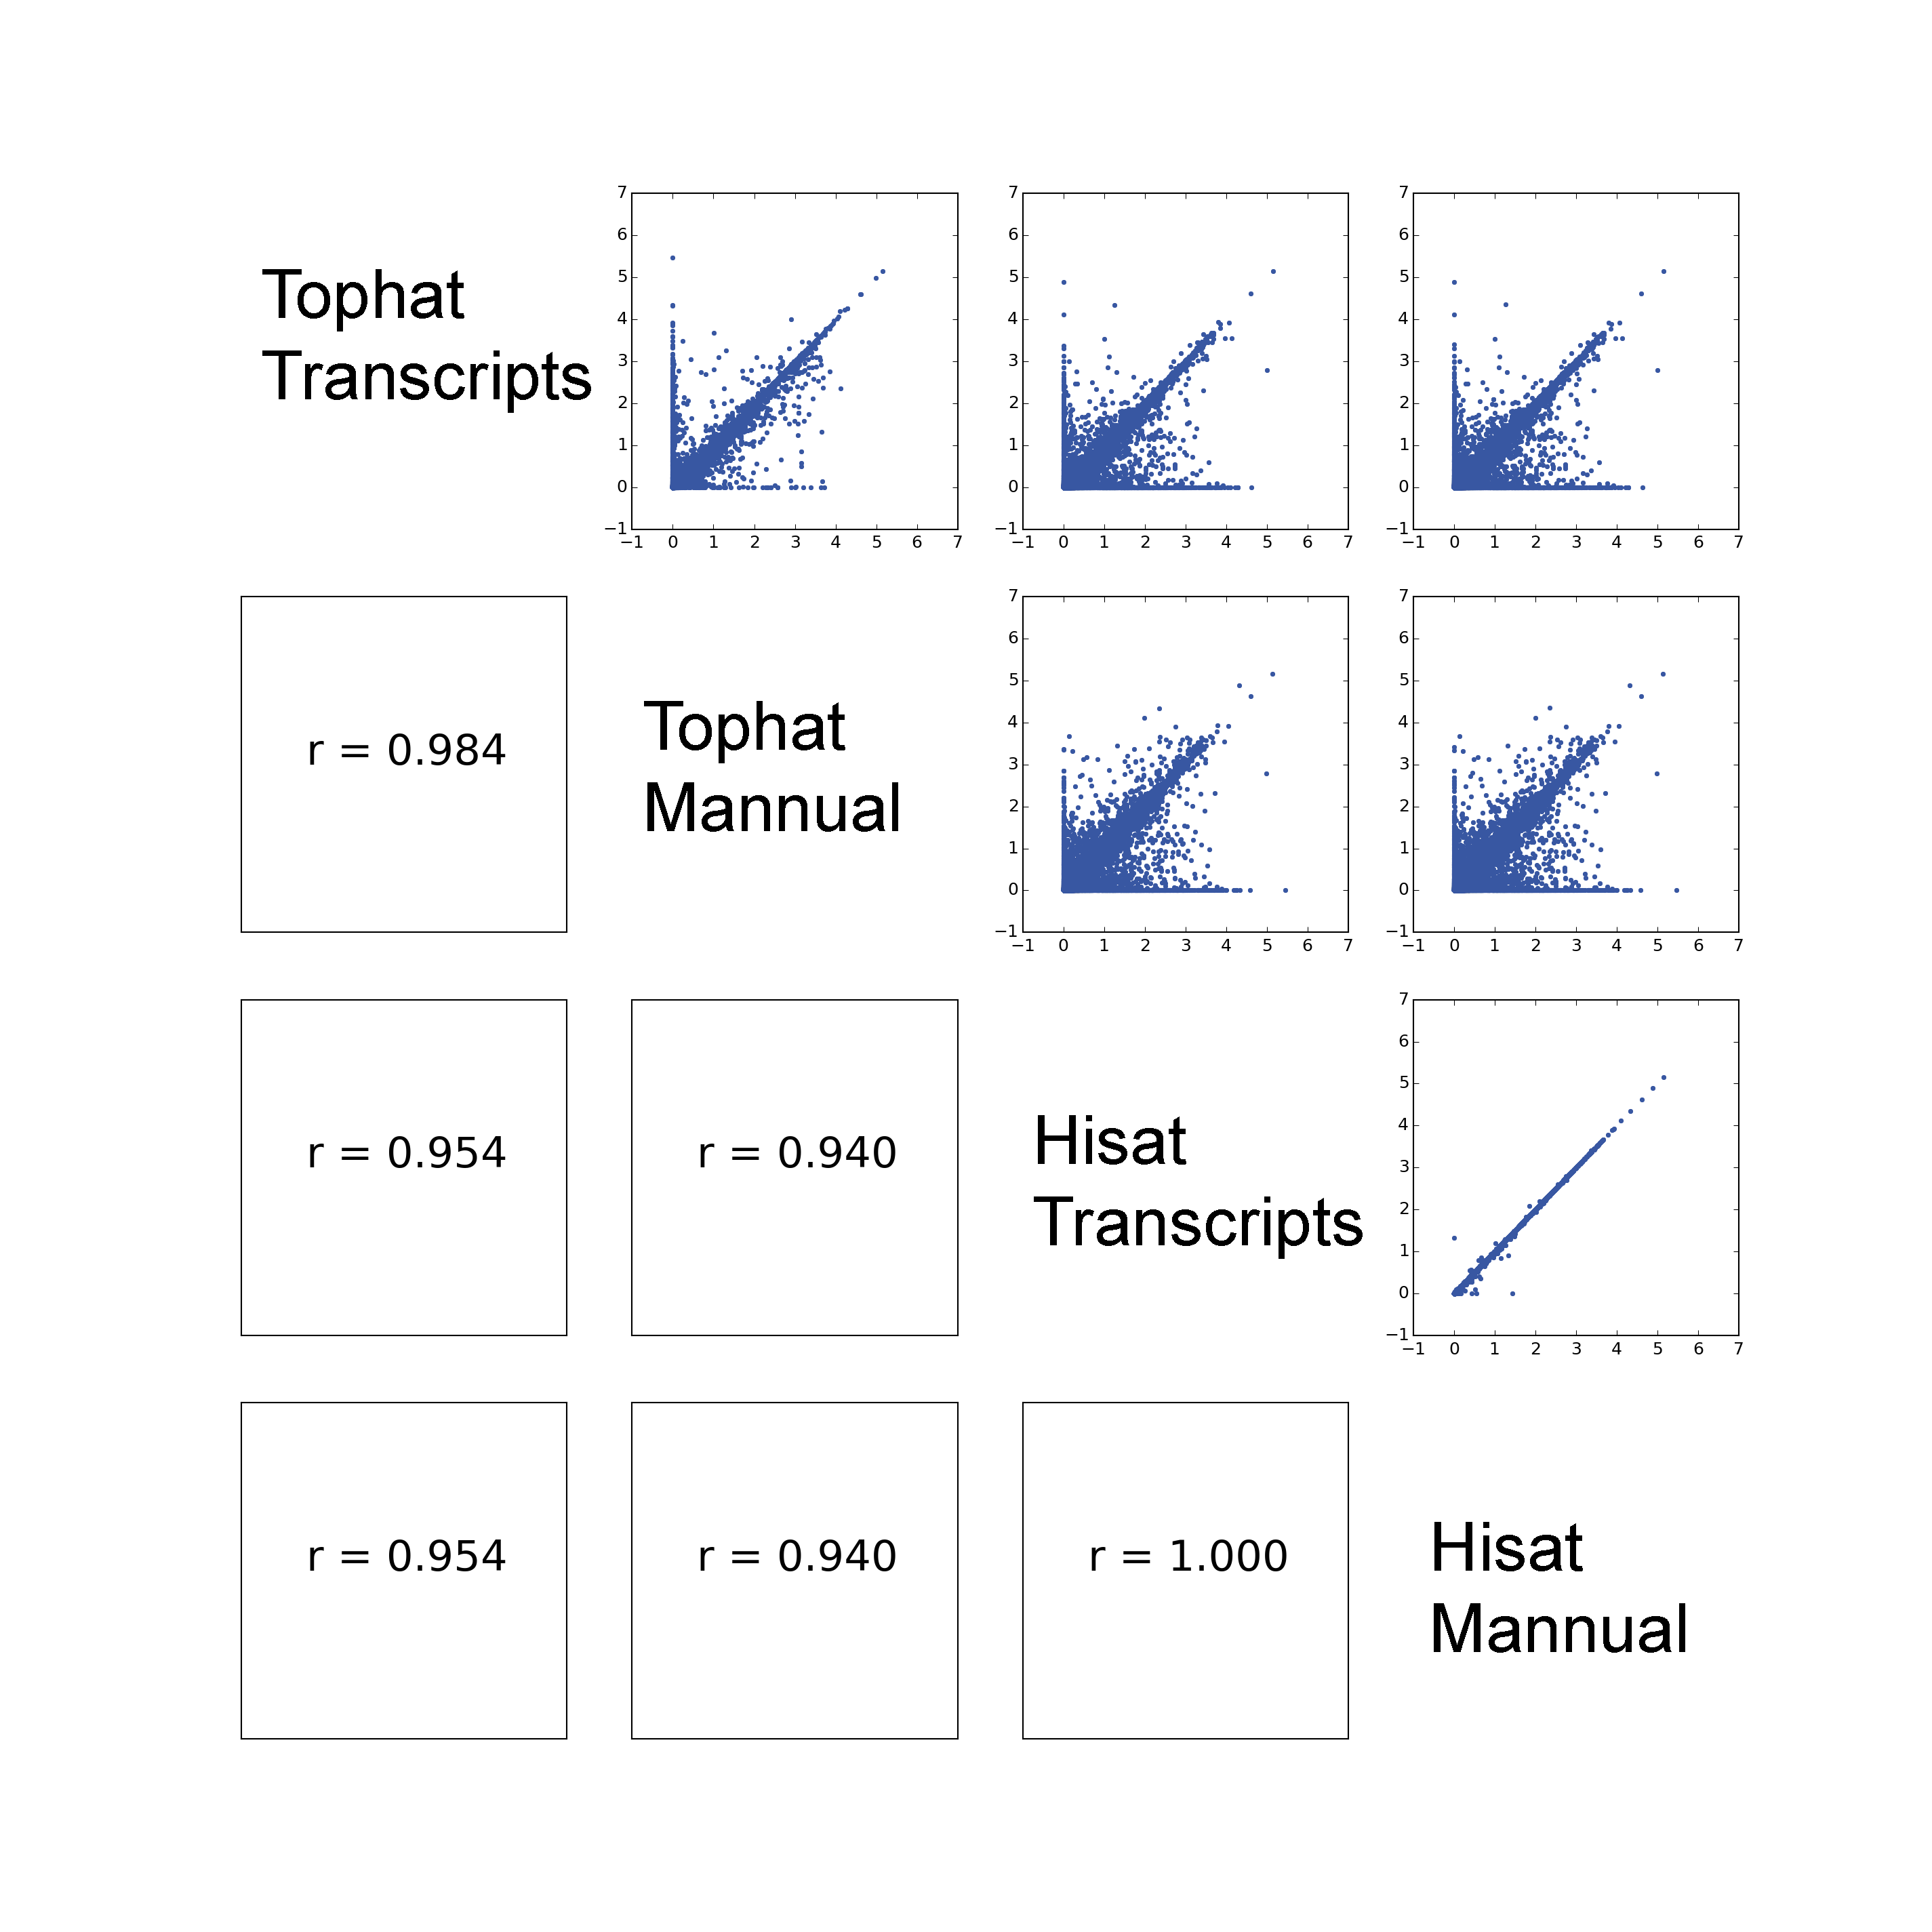
\includegraphics[height=4cm]{All_FPKM}	&  
				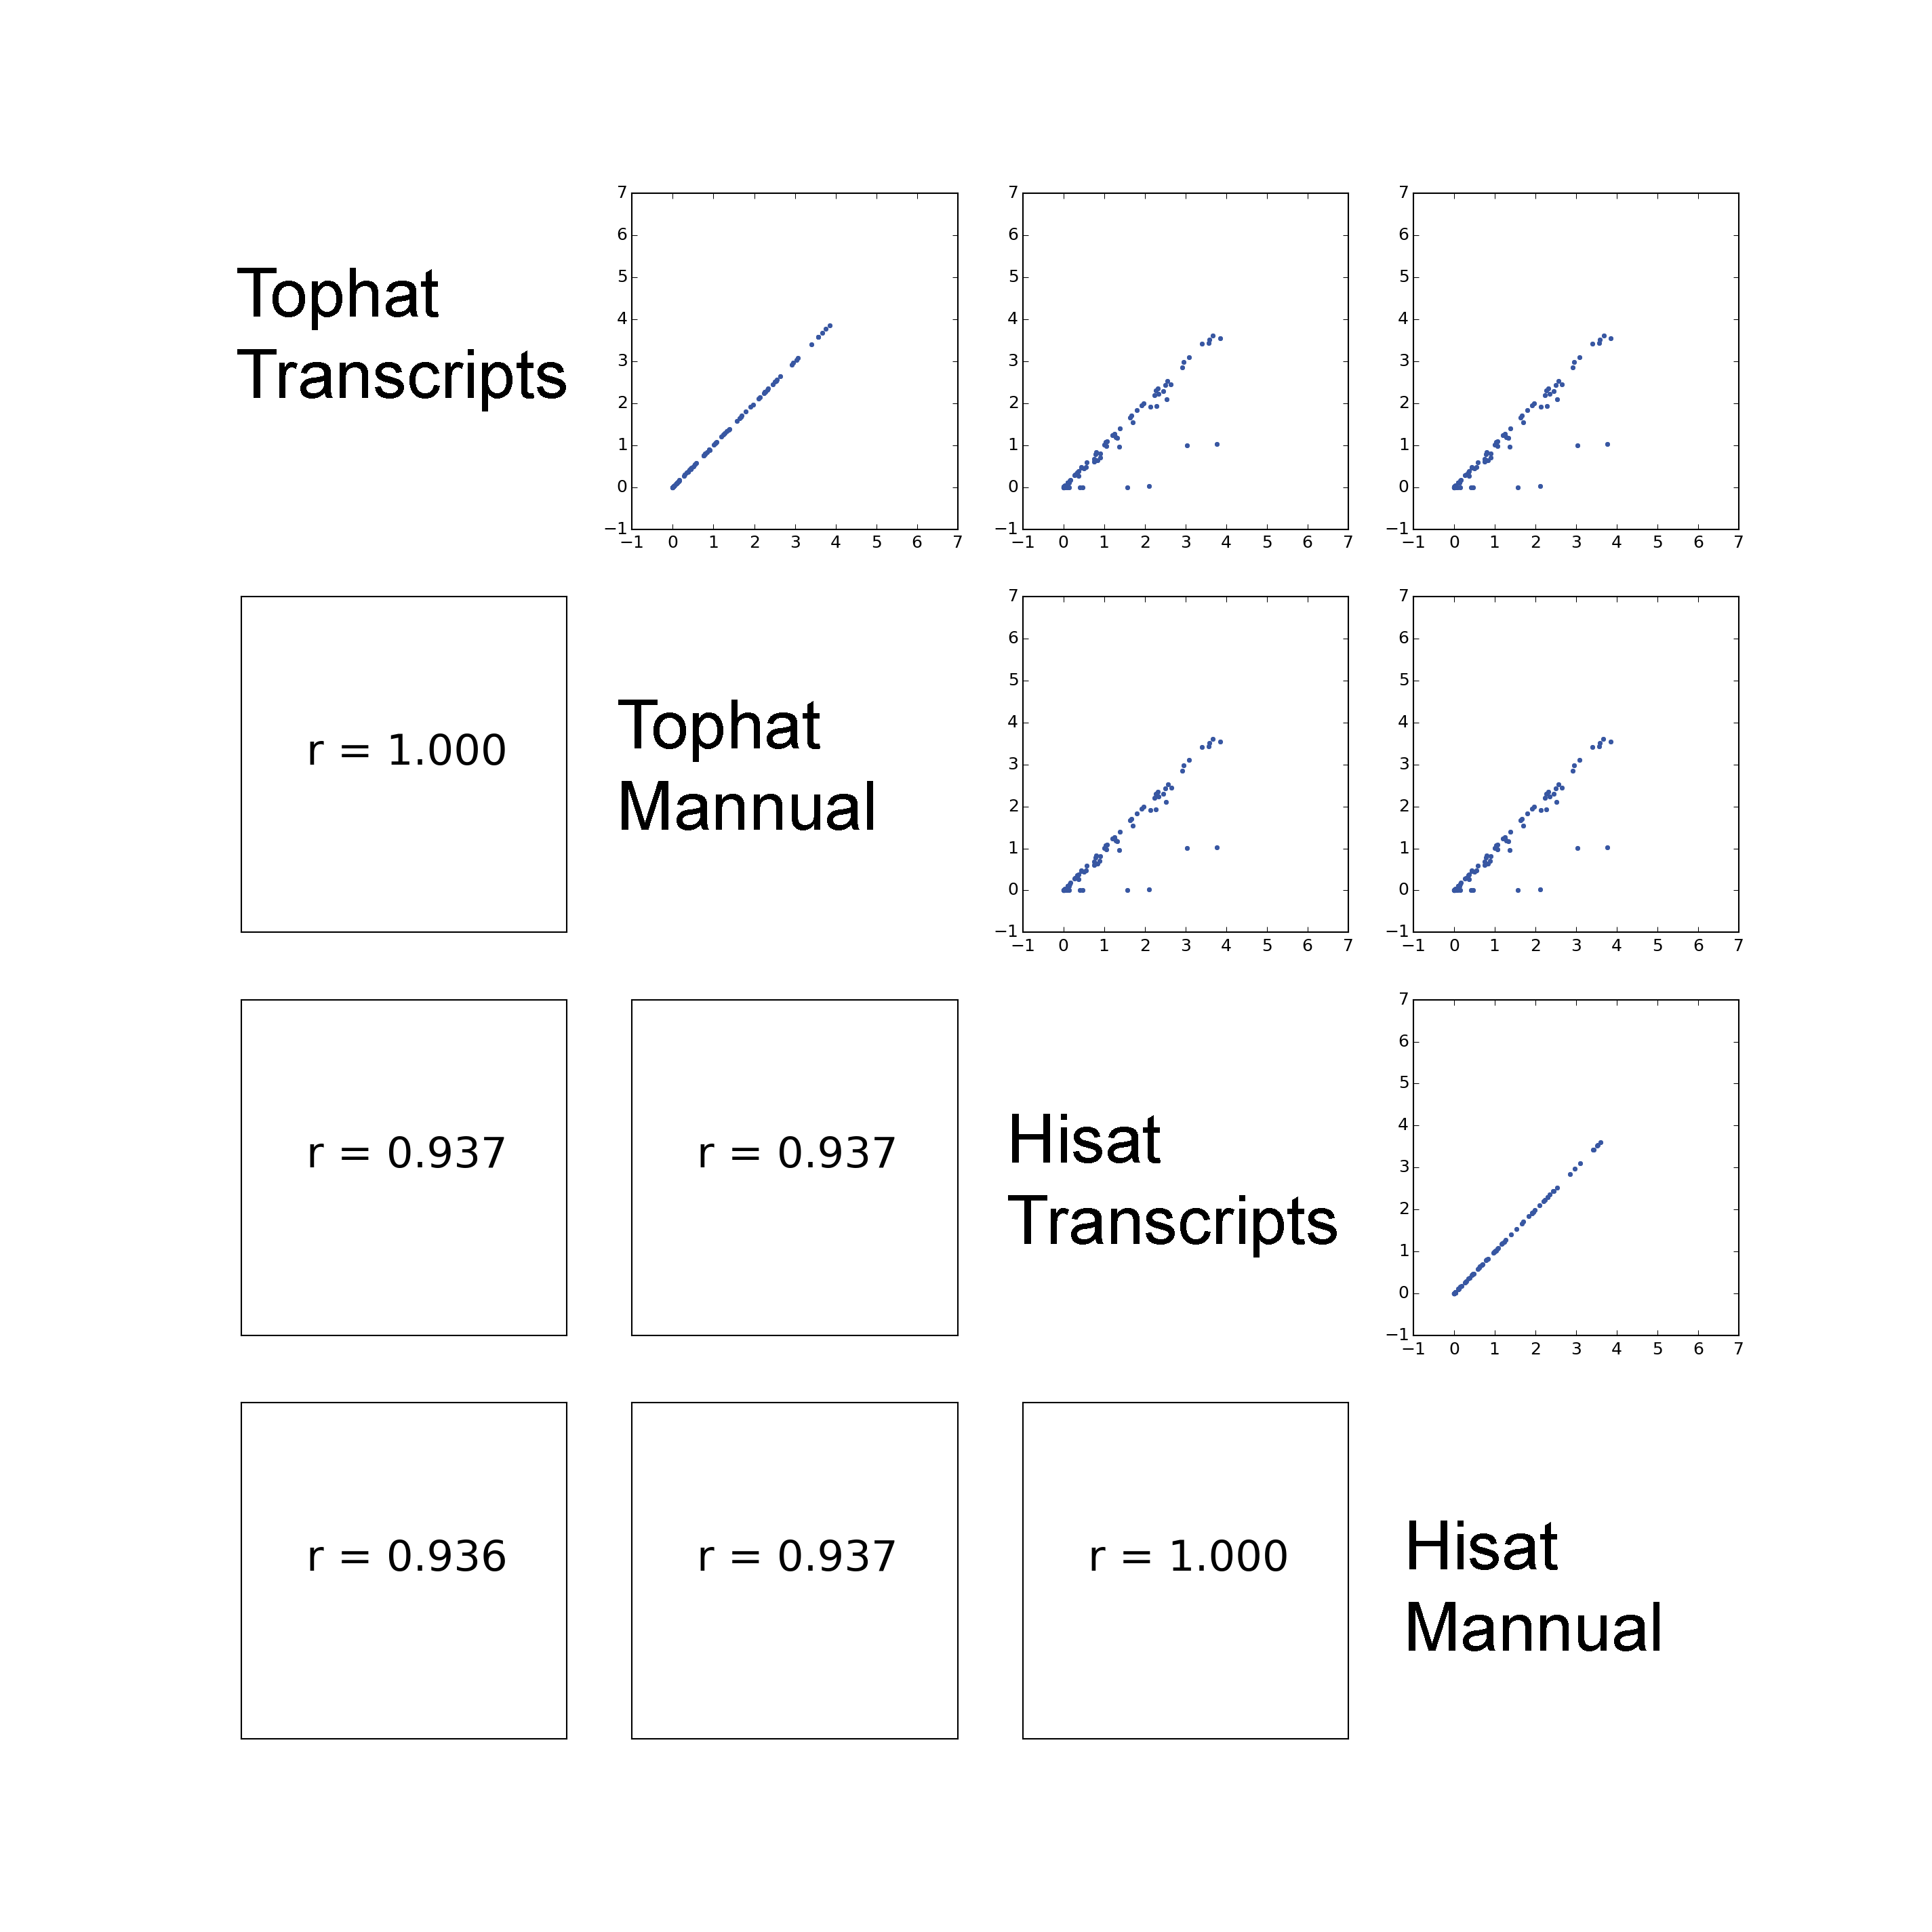
\includegraphics[height=4cm]{ERCC_FPKM}	\\	
			\end{tabular}	
			\end{table}	
			Higher for ERCC using Hisat.
	\end{block}
\end{frame}

\begin{frame}[c,fragile]
	\frametitle{ Result calculated by cuffquant-cuffnorm. }
	\begin{block}{ FPKM for Refseq genes and Noncode v4 transcripts. }
			\begin{table}
			\centering	
			\begin{tabular}{C{4cm}  C{4cm}}     
				Refseq genes		& Noncode v4 	\\
				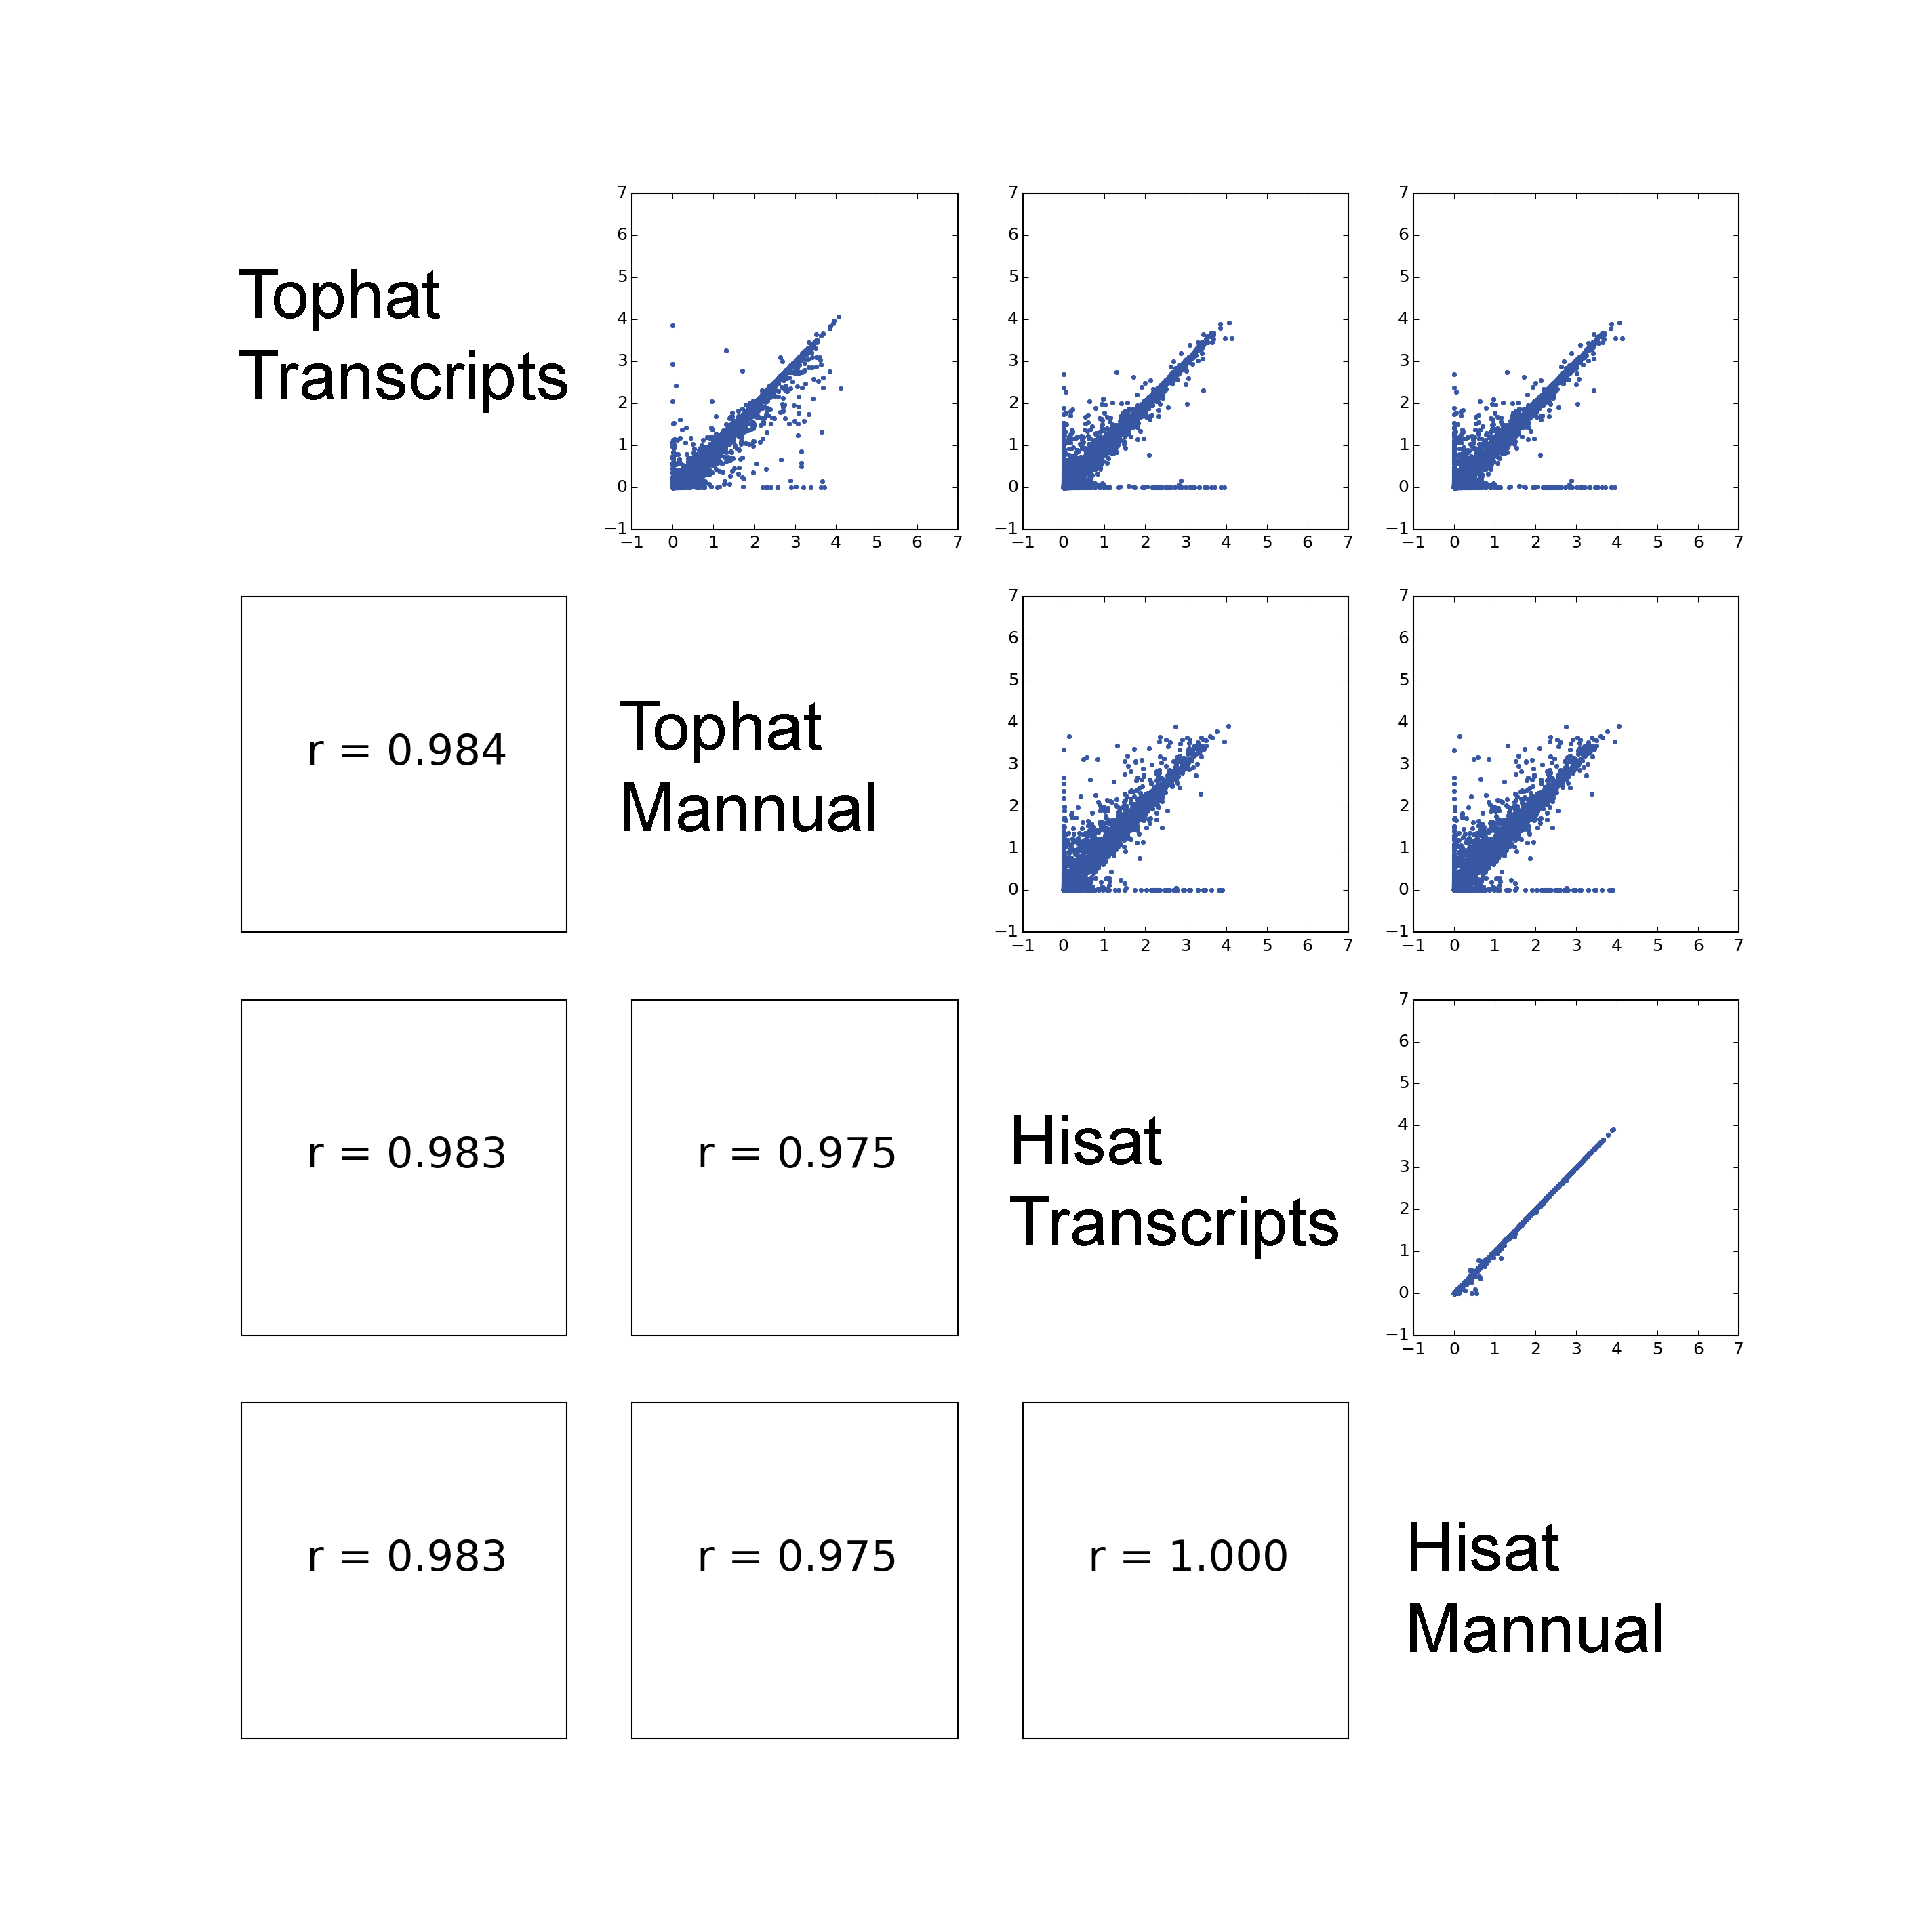
\includegraphics[height=4cm]{Refgene_FPKM}	&  
				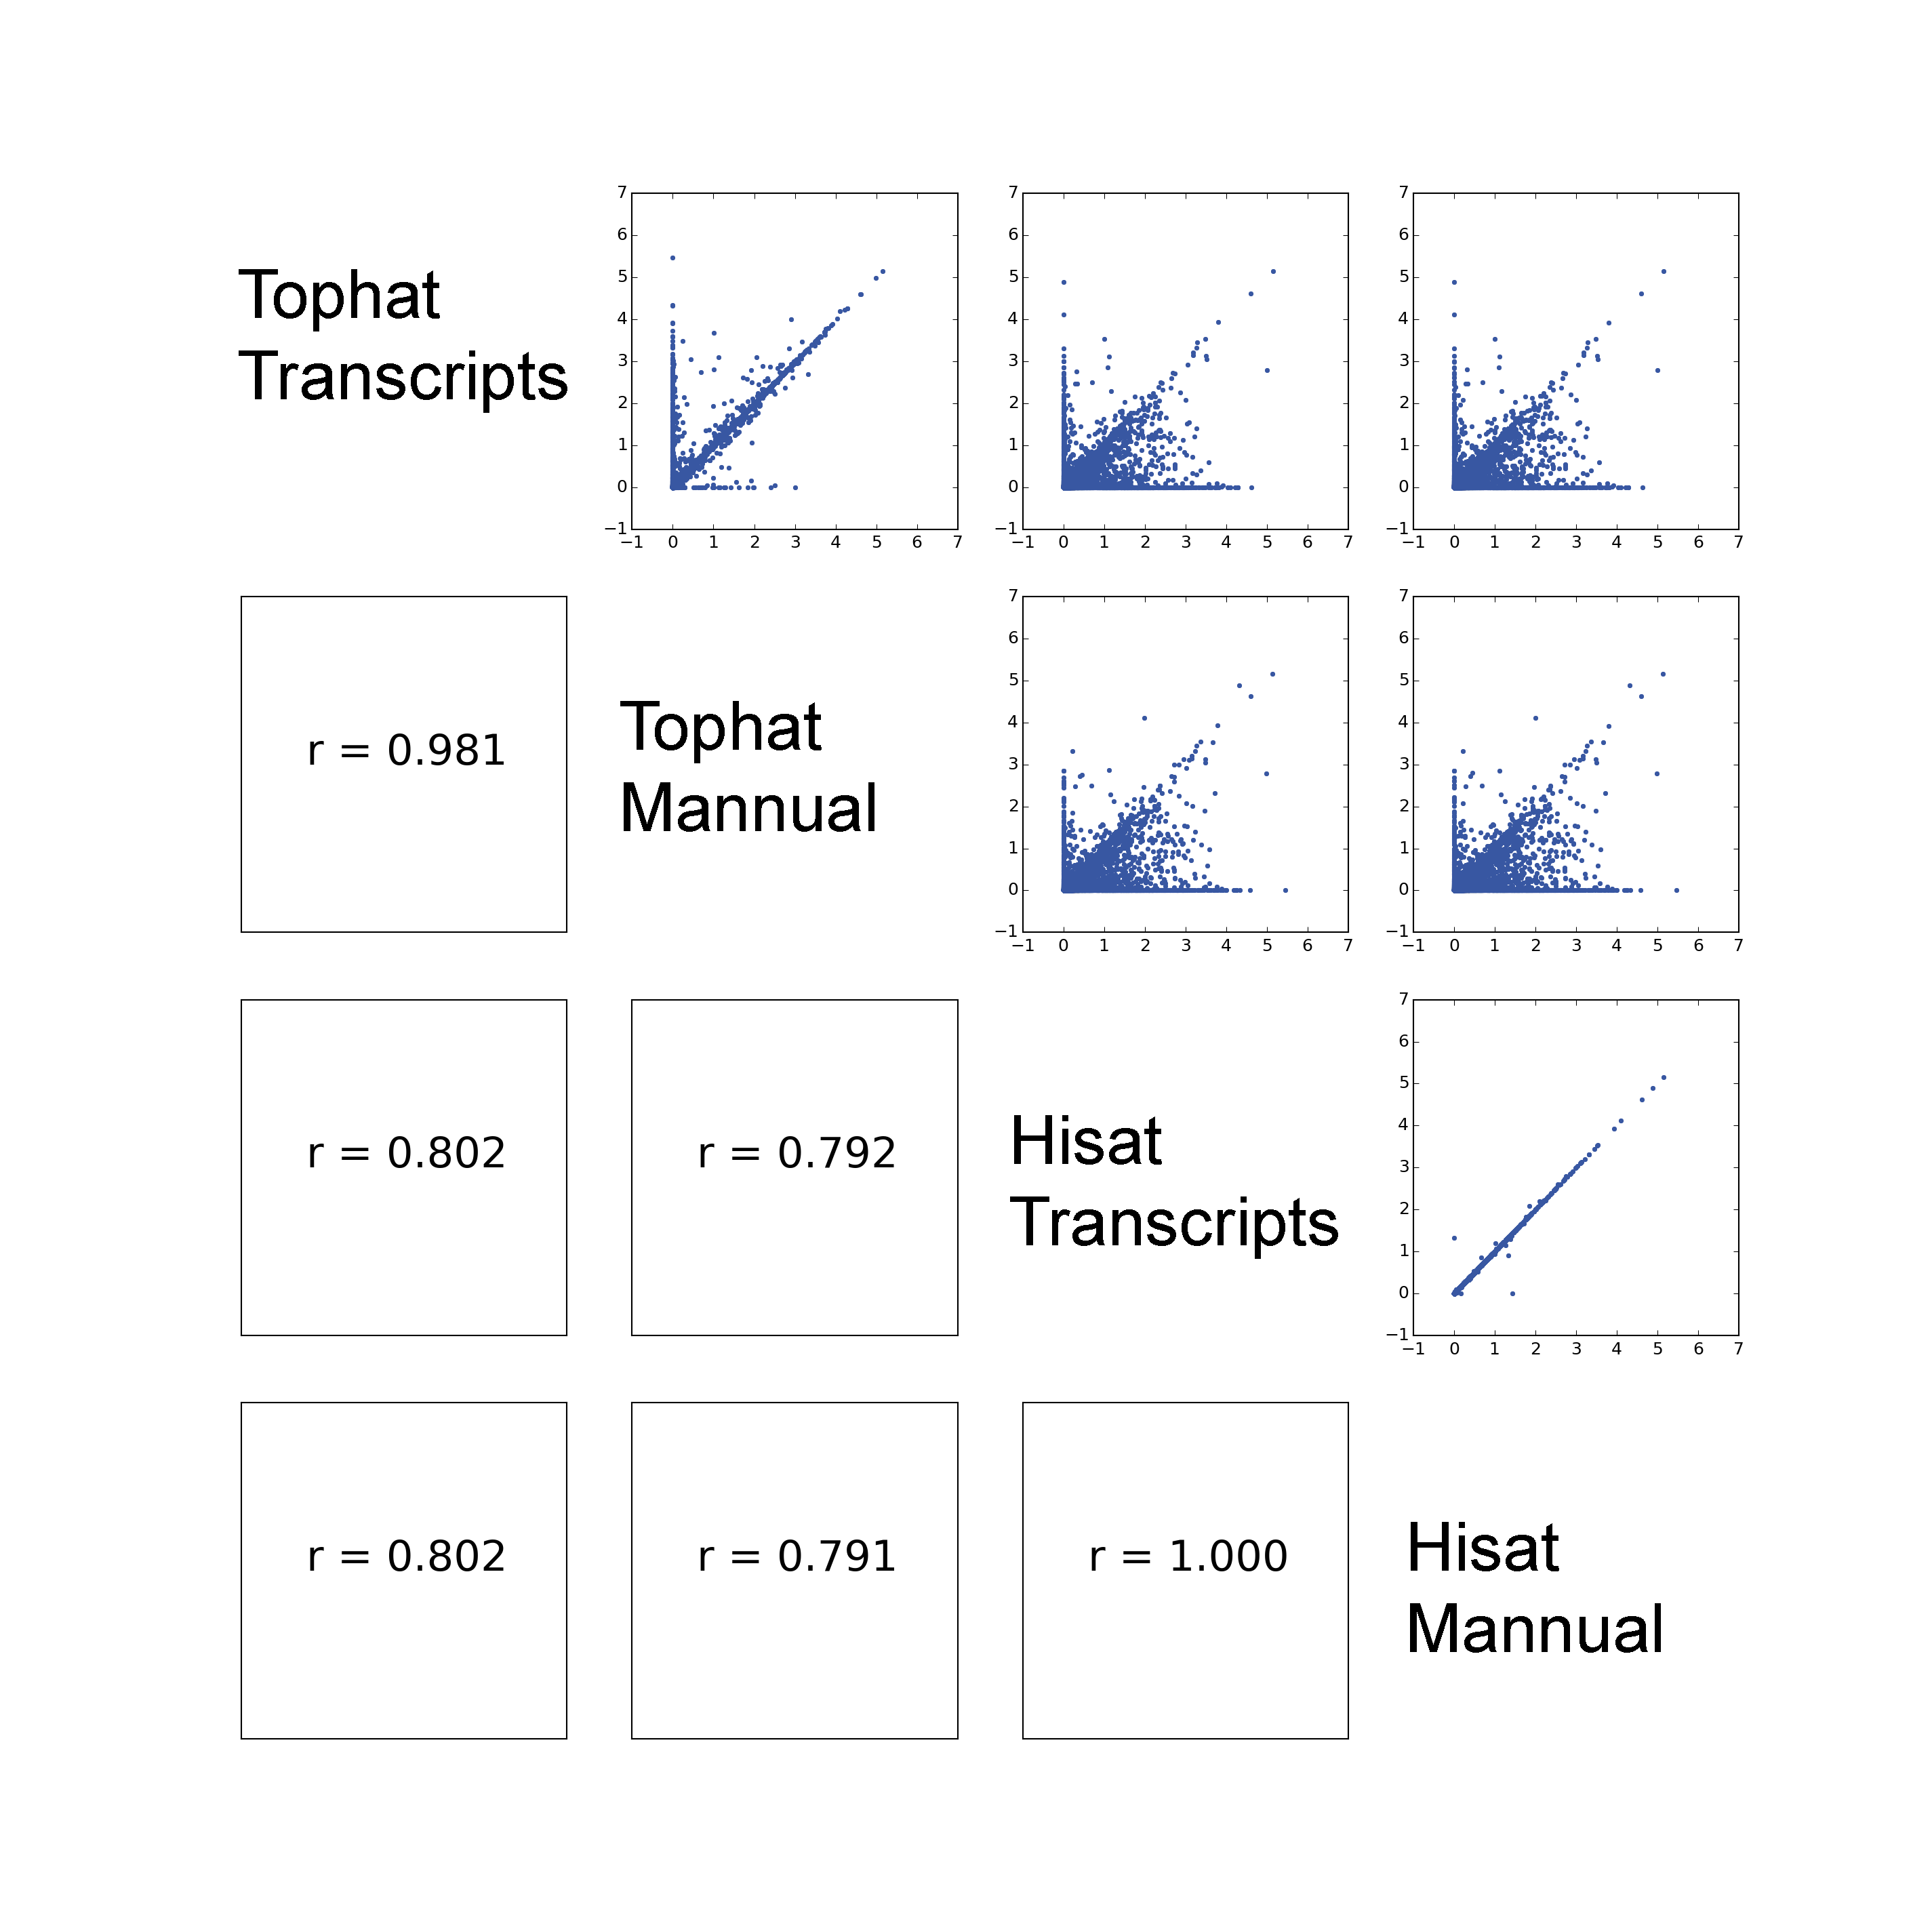
\includegraphics[height=4cm]{NONCODE_FPKM}	\\	
			\end{tabular}	
			\end{table}	
	\end{block}
\end{frame}

\begin{frame}[c,fragile]
	\frametitle{ Refseq: (((HT,HM),TM),TT); ERCC: almost the same. }
	\begin{block}{ Read Counts for refseq-genes. }
			\begin{table}
			\centering	
			\begin{tabular}{C{4cm}  C{4cm}}     
				Refseq genes		& ERCC spike-ins 	\\
				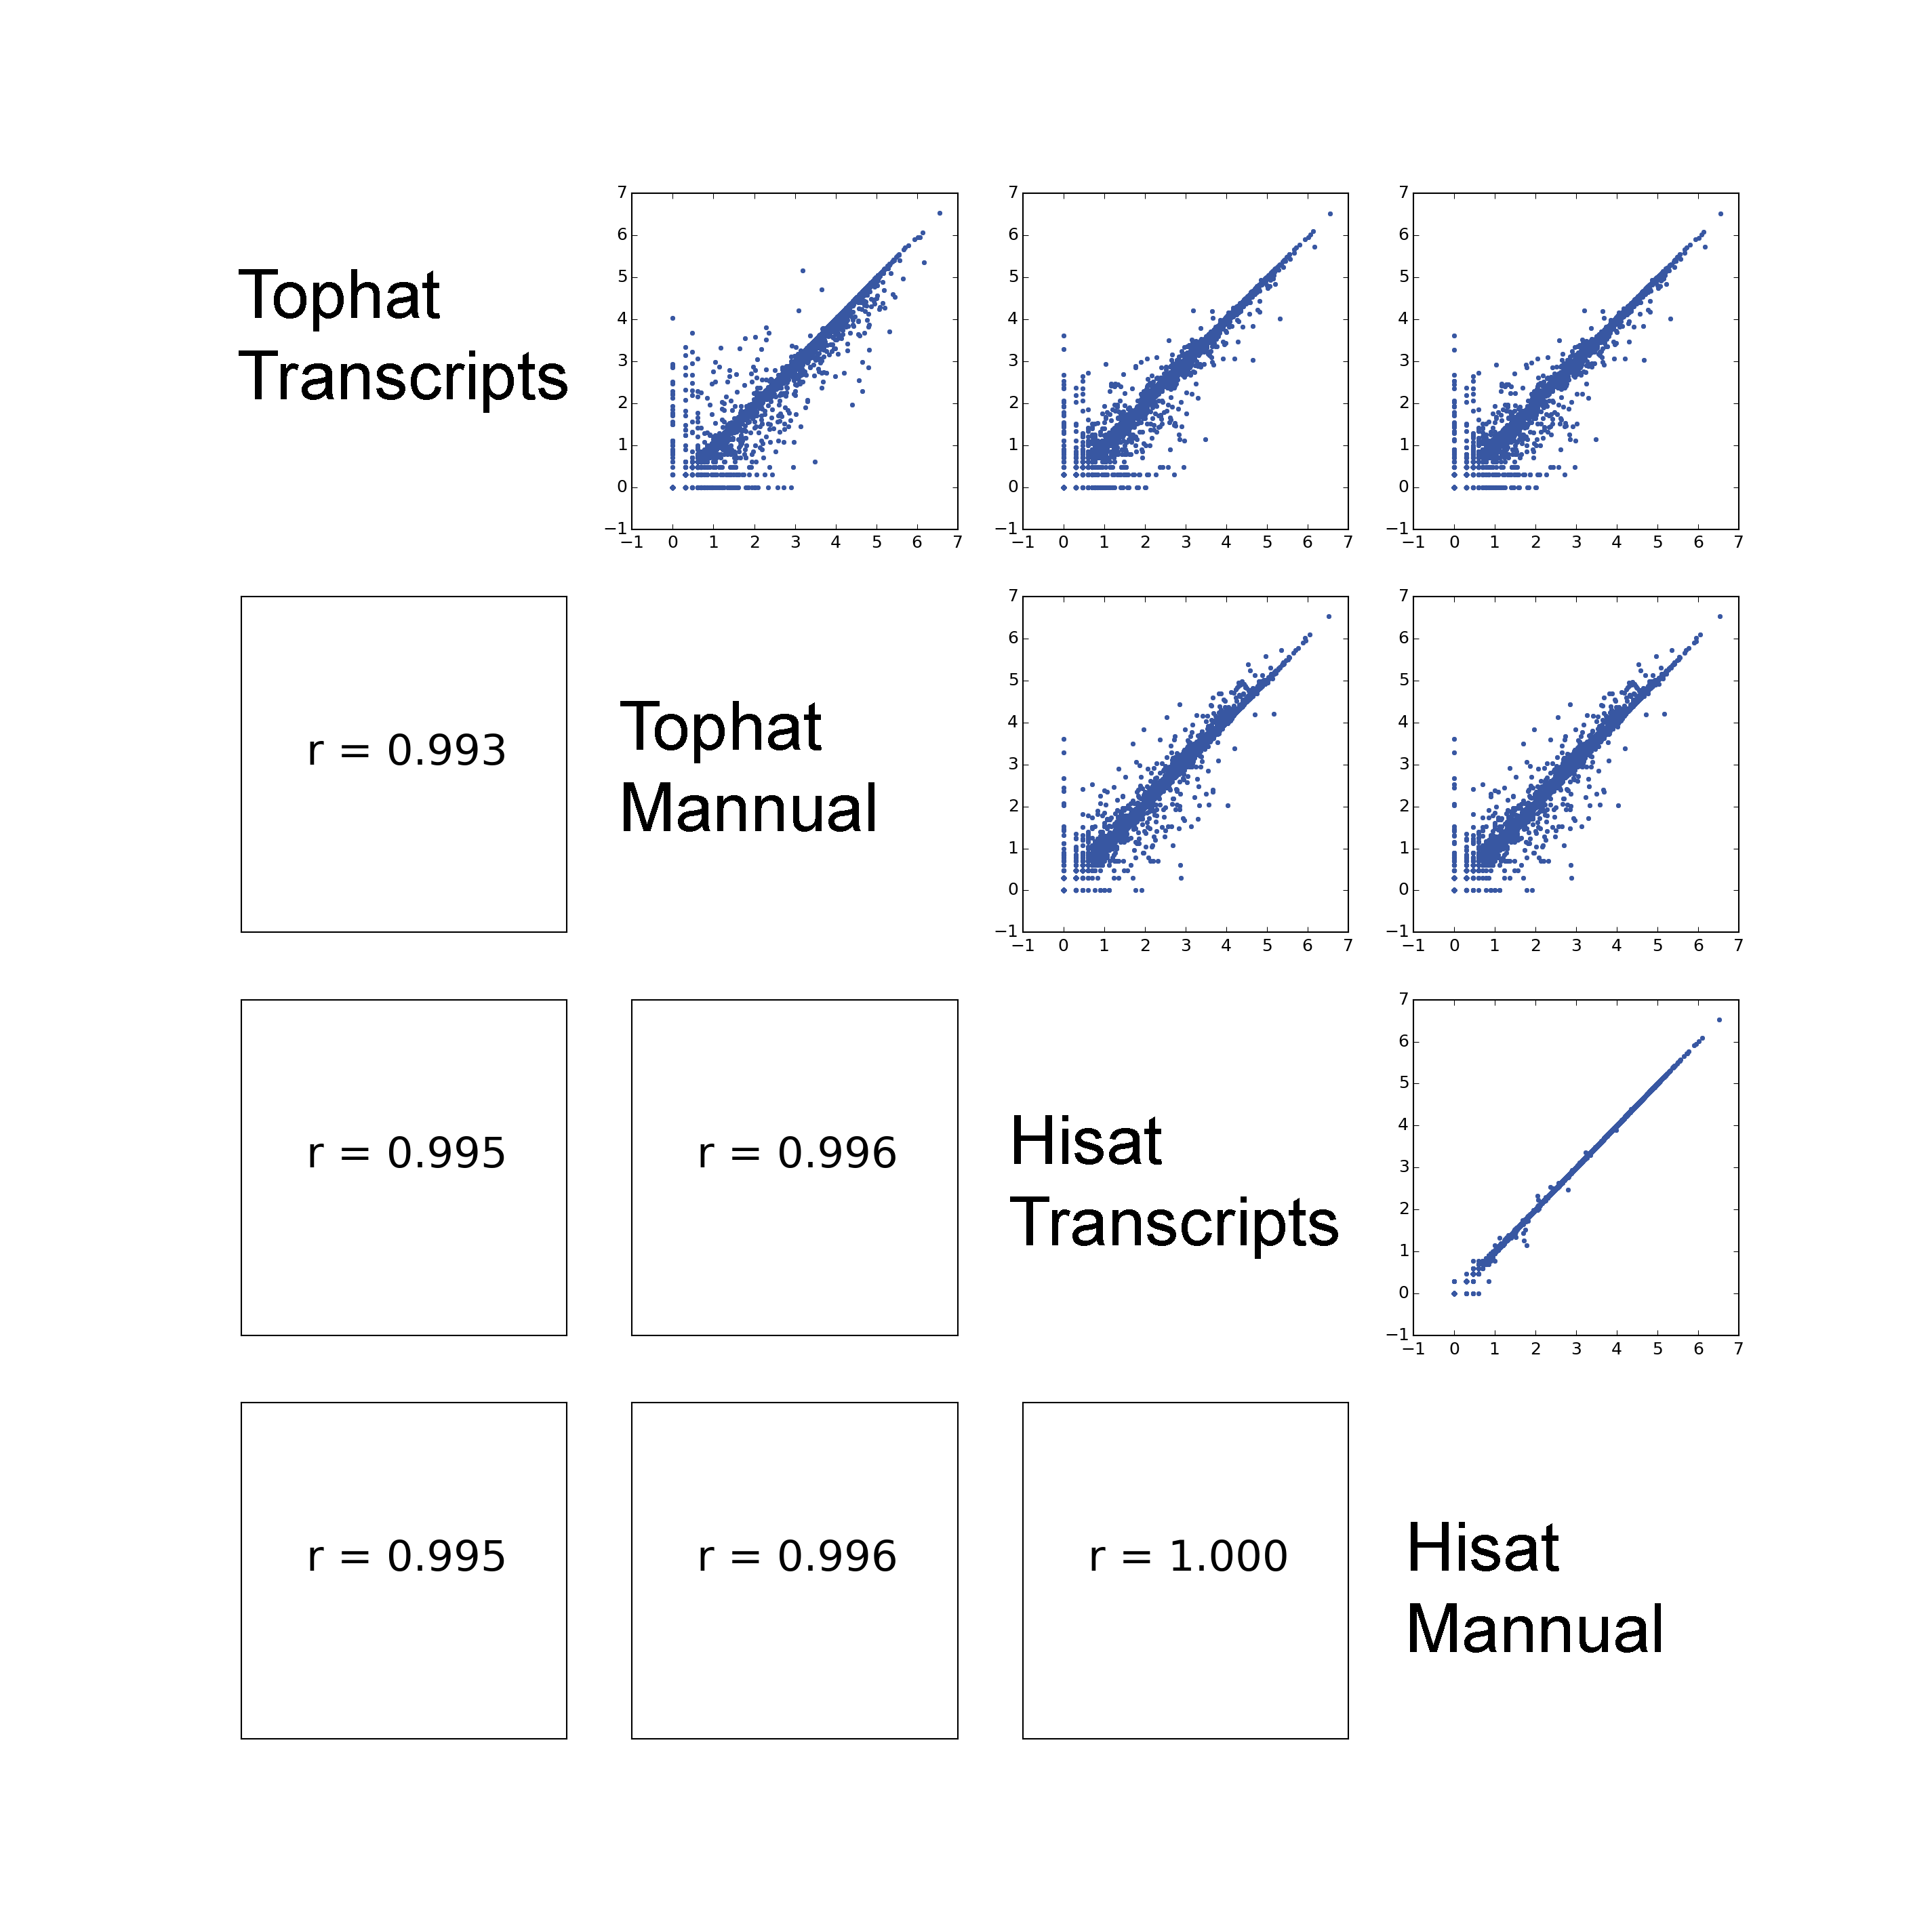
\includegraphics[height=4cm]{Refseq_count}	&  
				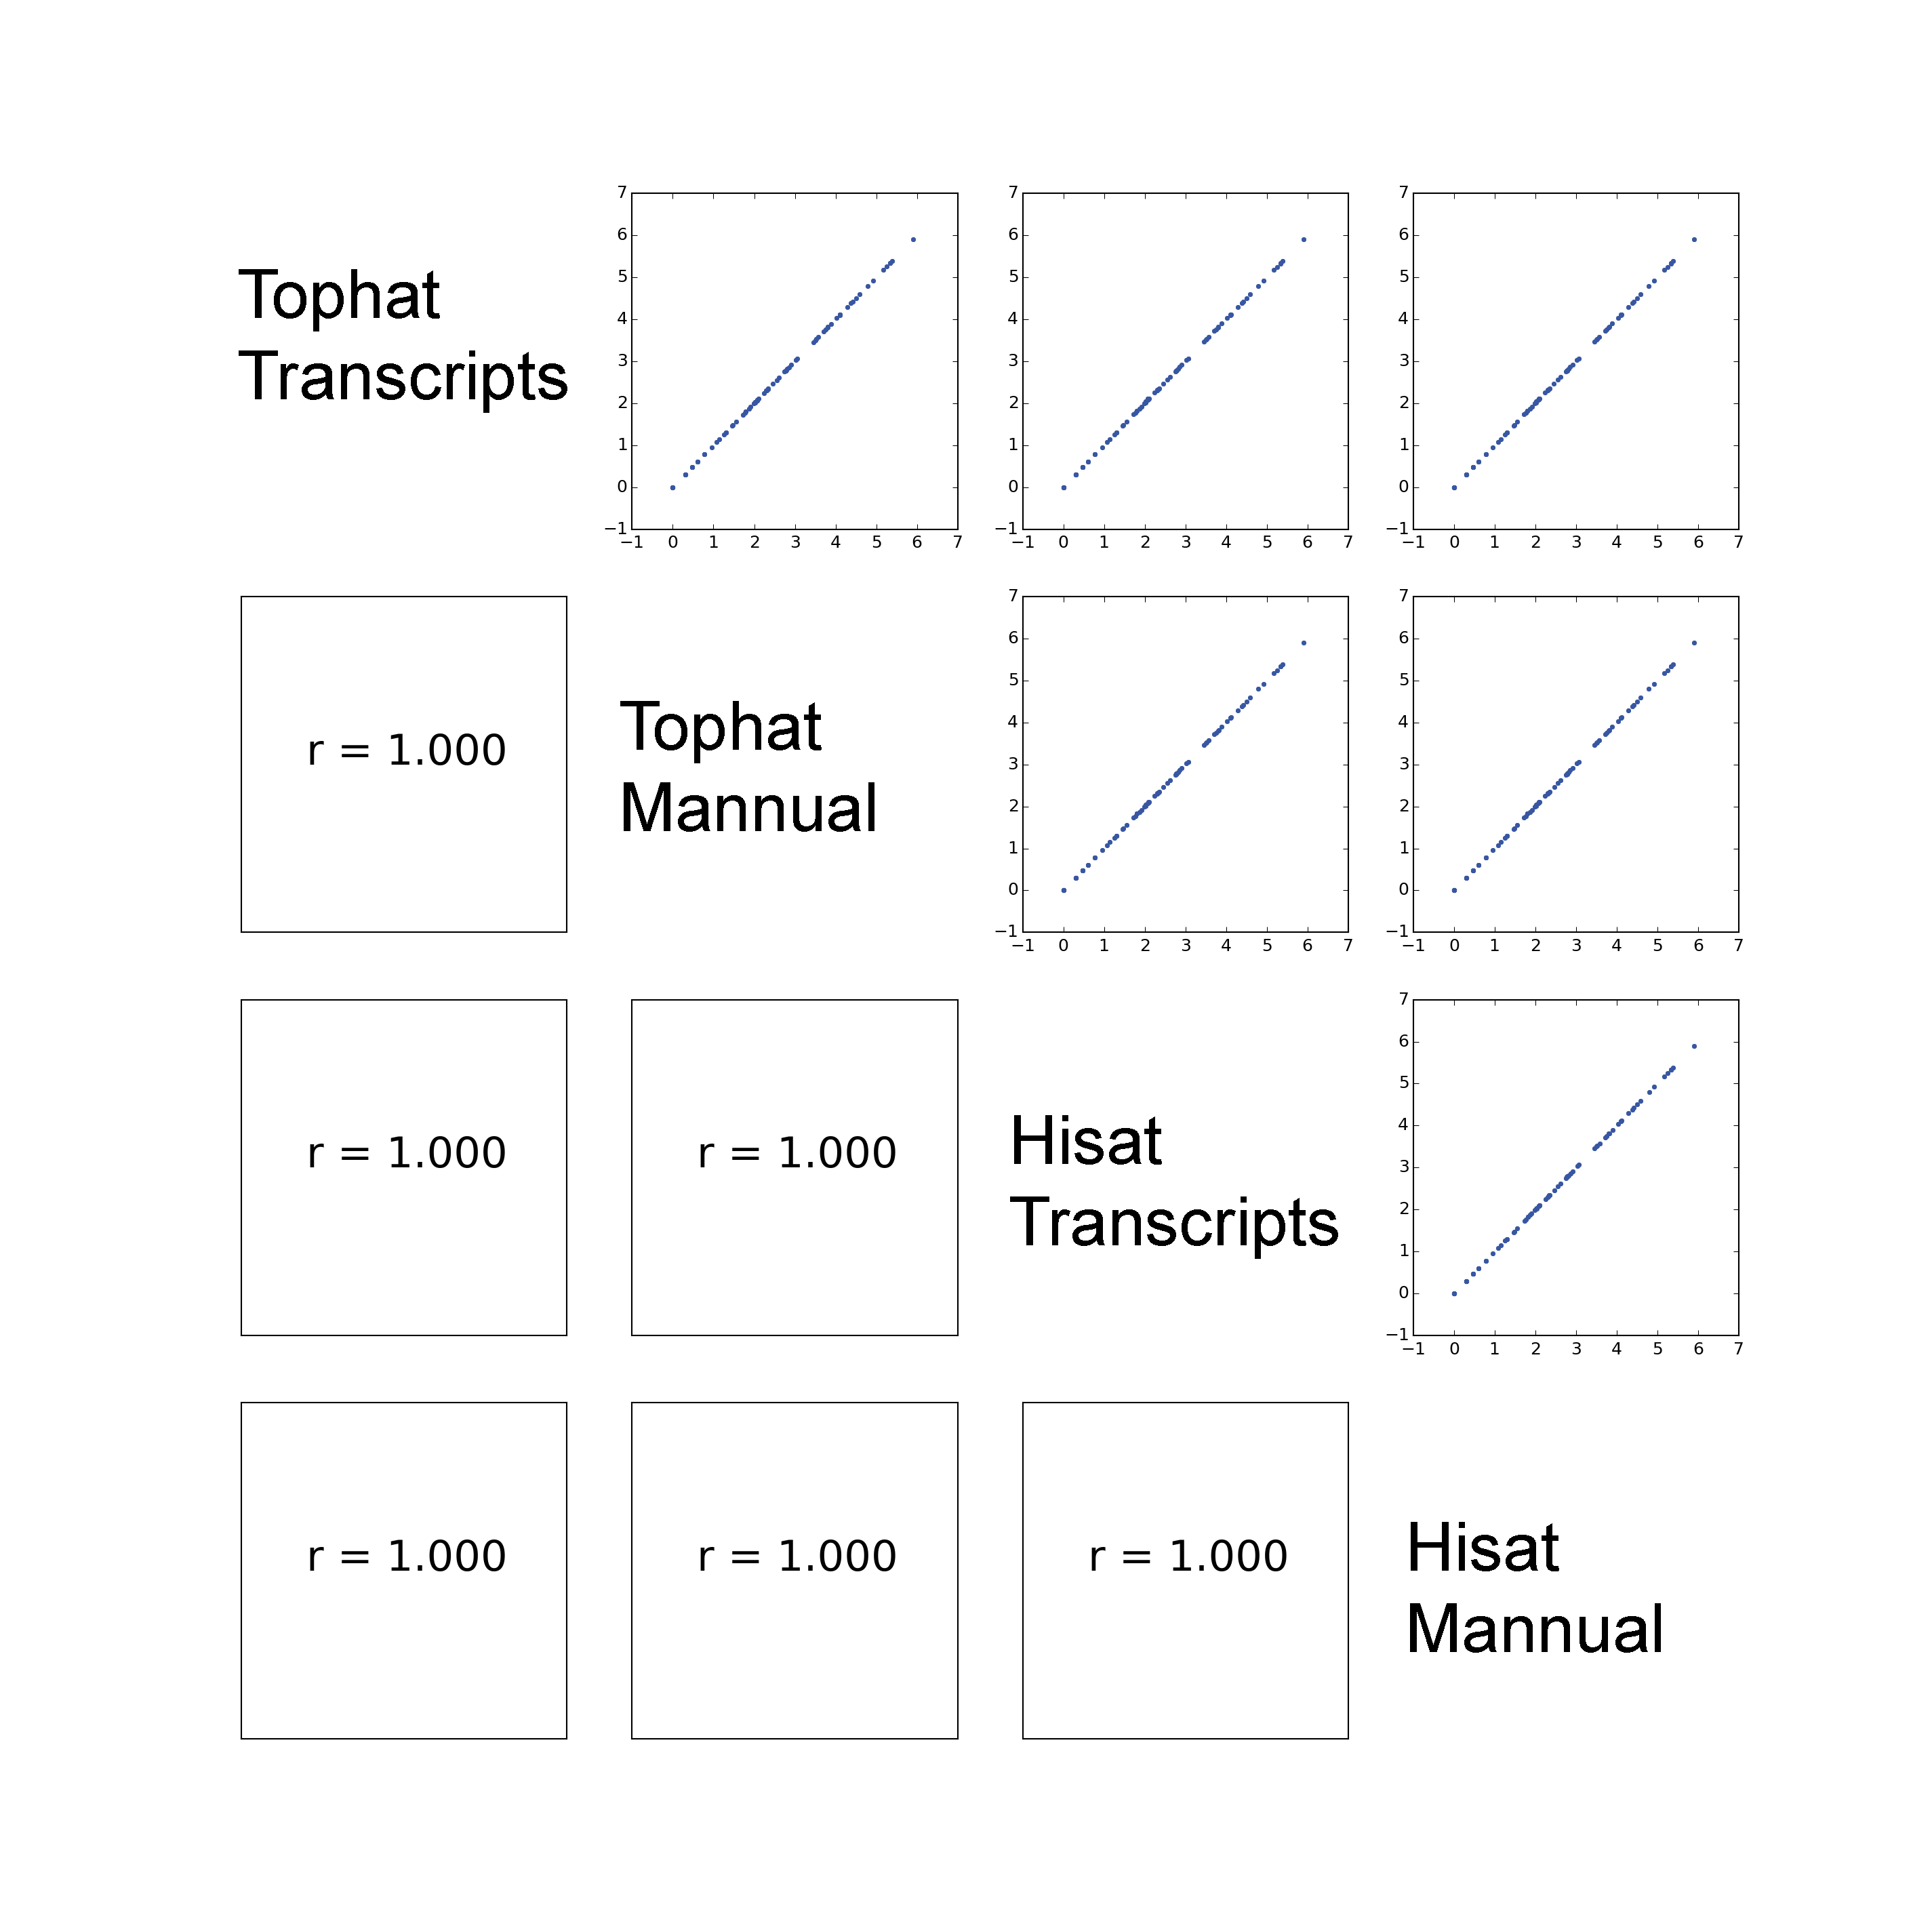
\includegraphics[height=4cm]{ERCC_count}	\\	
			\end{tabular}	
			\end{table}	
			\tiny{Why Hisat FPKM were higher but HTSeq unique count were almost the same? \\ \pause
			Hisat could find more multiple alignments. ERCC contained some repeat sequences.}
	\end{block}
\end{frame}


\begin{frame}[c,fragile]
	\frametitle{ Linc-RNA detection: TT $>$ TM $>$ HT = HM. }
	\begin{block}{ Read Counts for refseq-genes. }
			\begin{table}
			\centering	
			\begin{tabular}{C{3cm} C{3cm} C{3cm}}     
				Noncode 4.0		& nsmb 2660 & novo lincRNA 	\\
				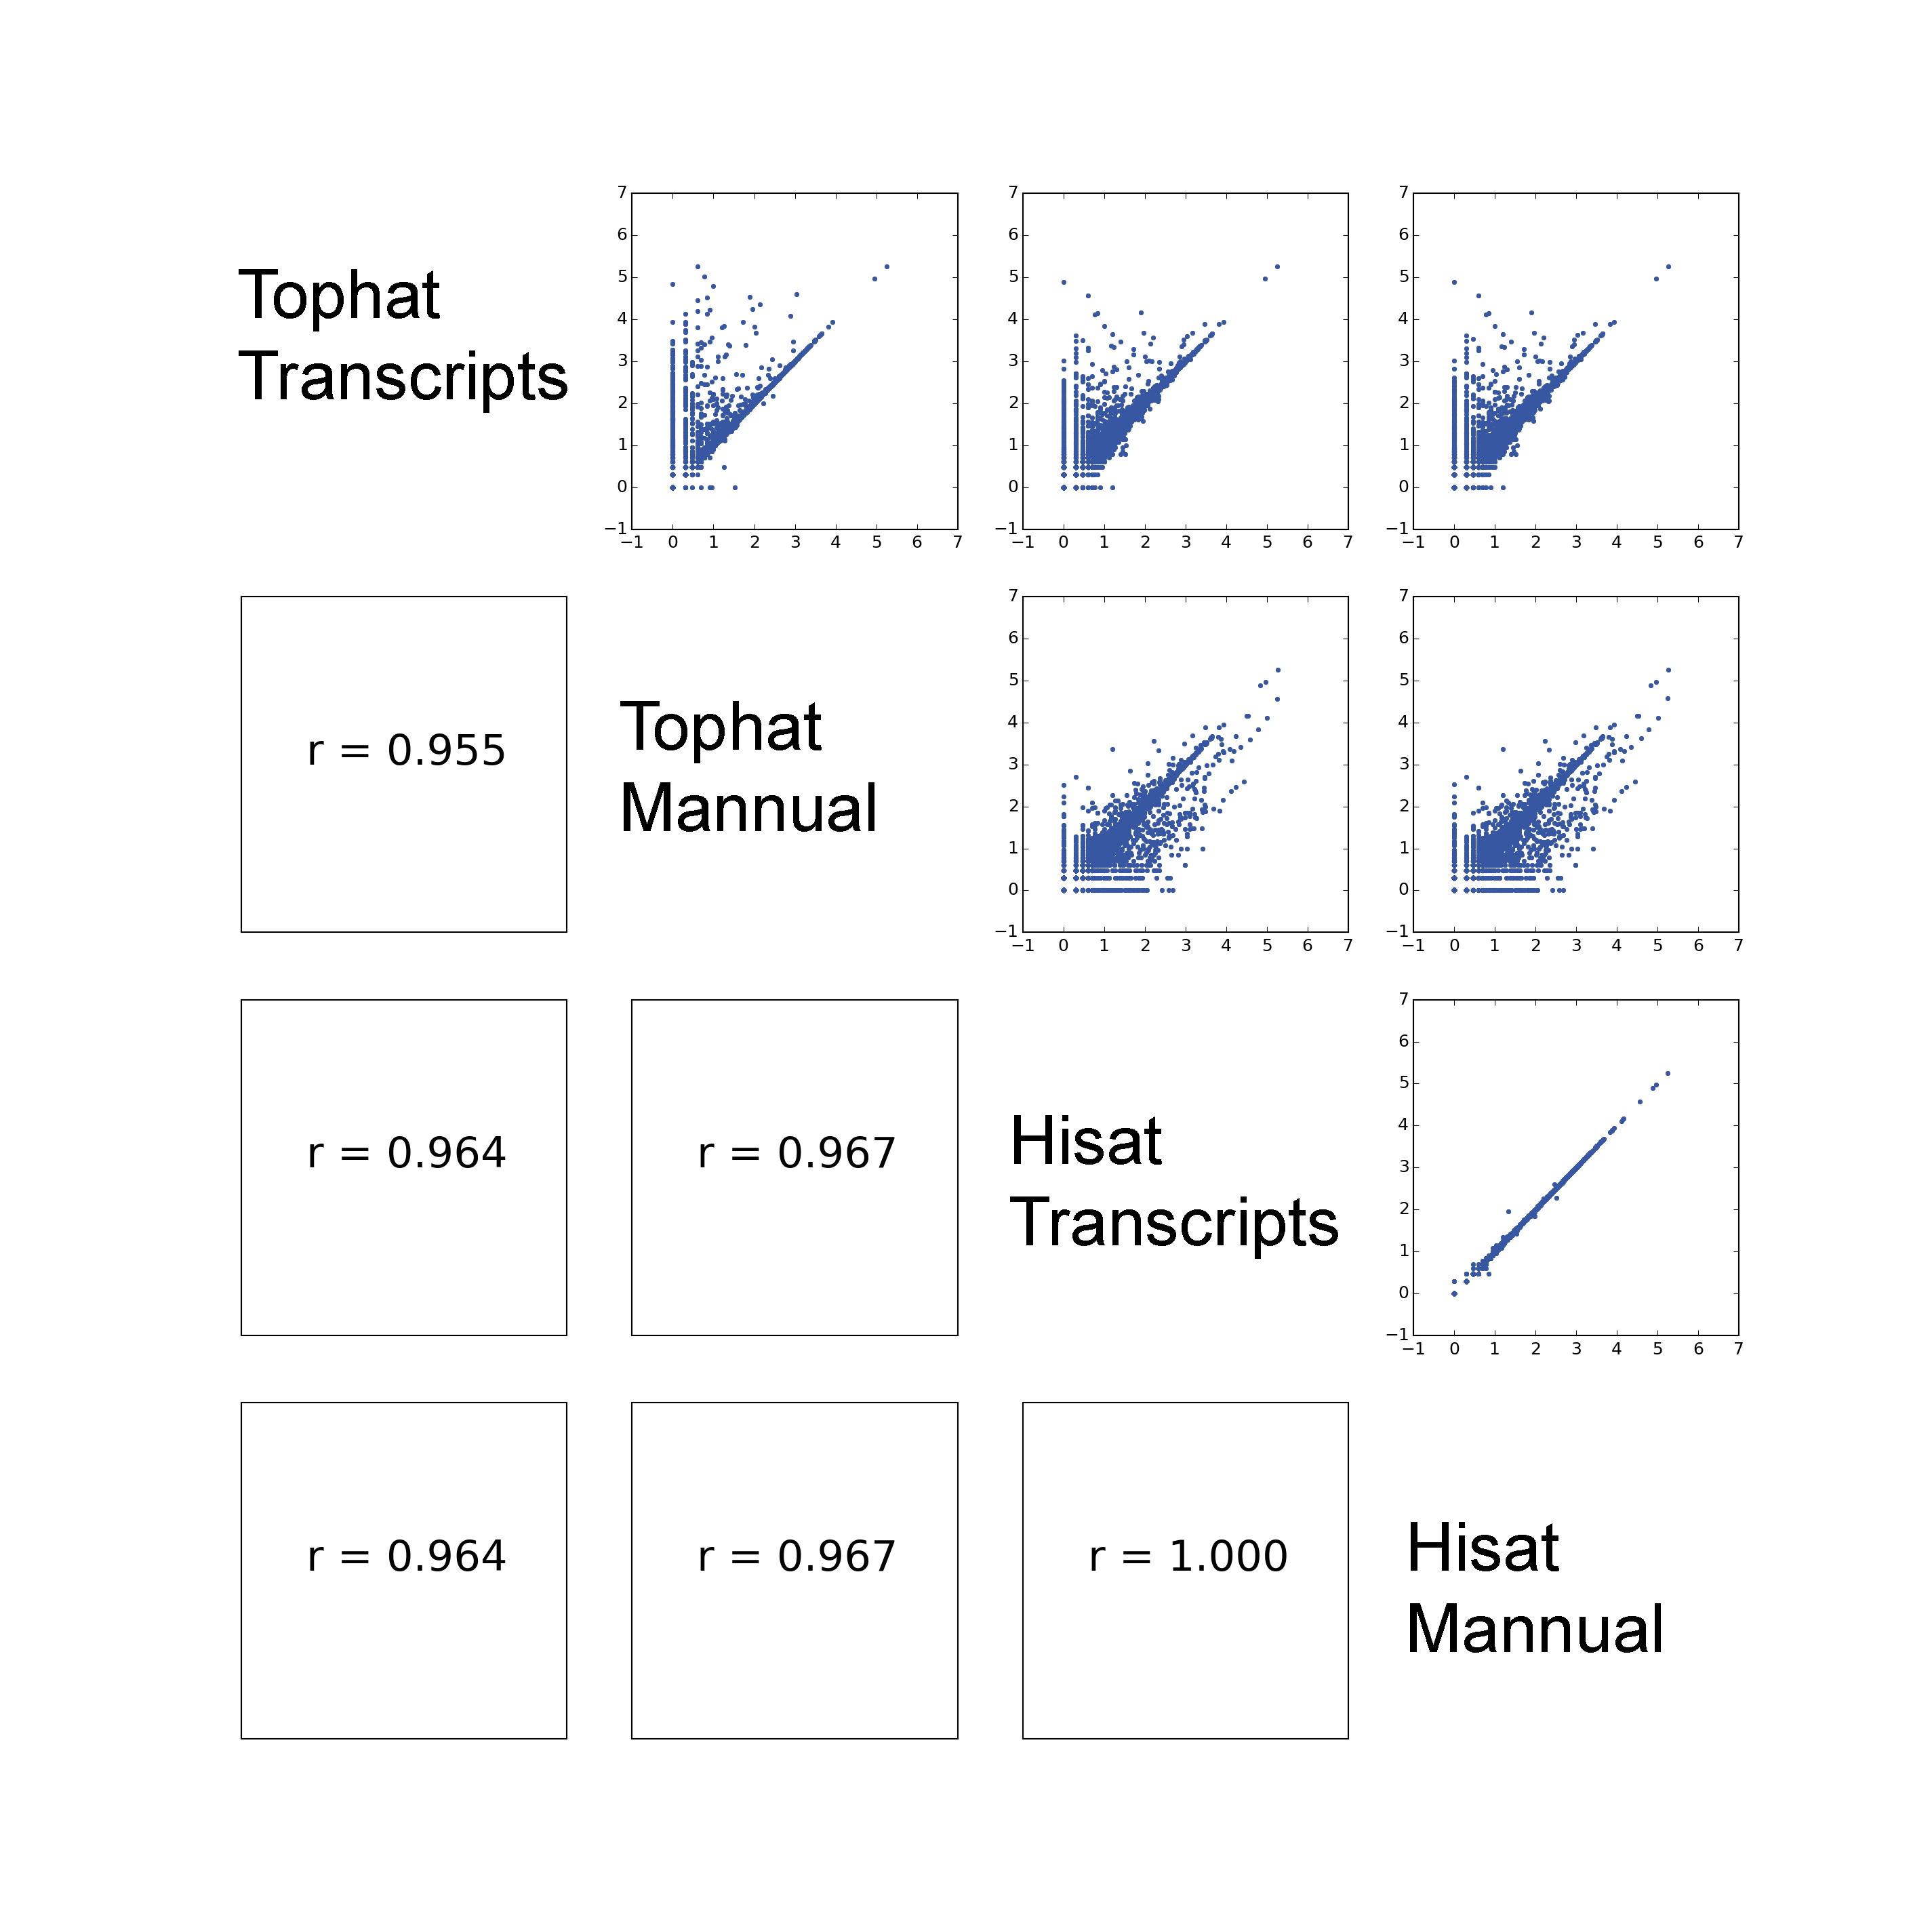
\includegraphics[height=3cm ]{Noncode_count} &  
				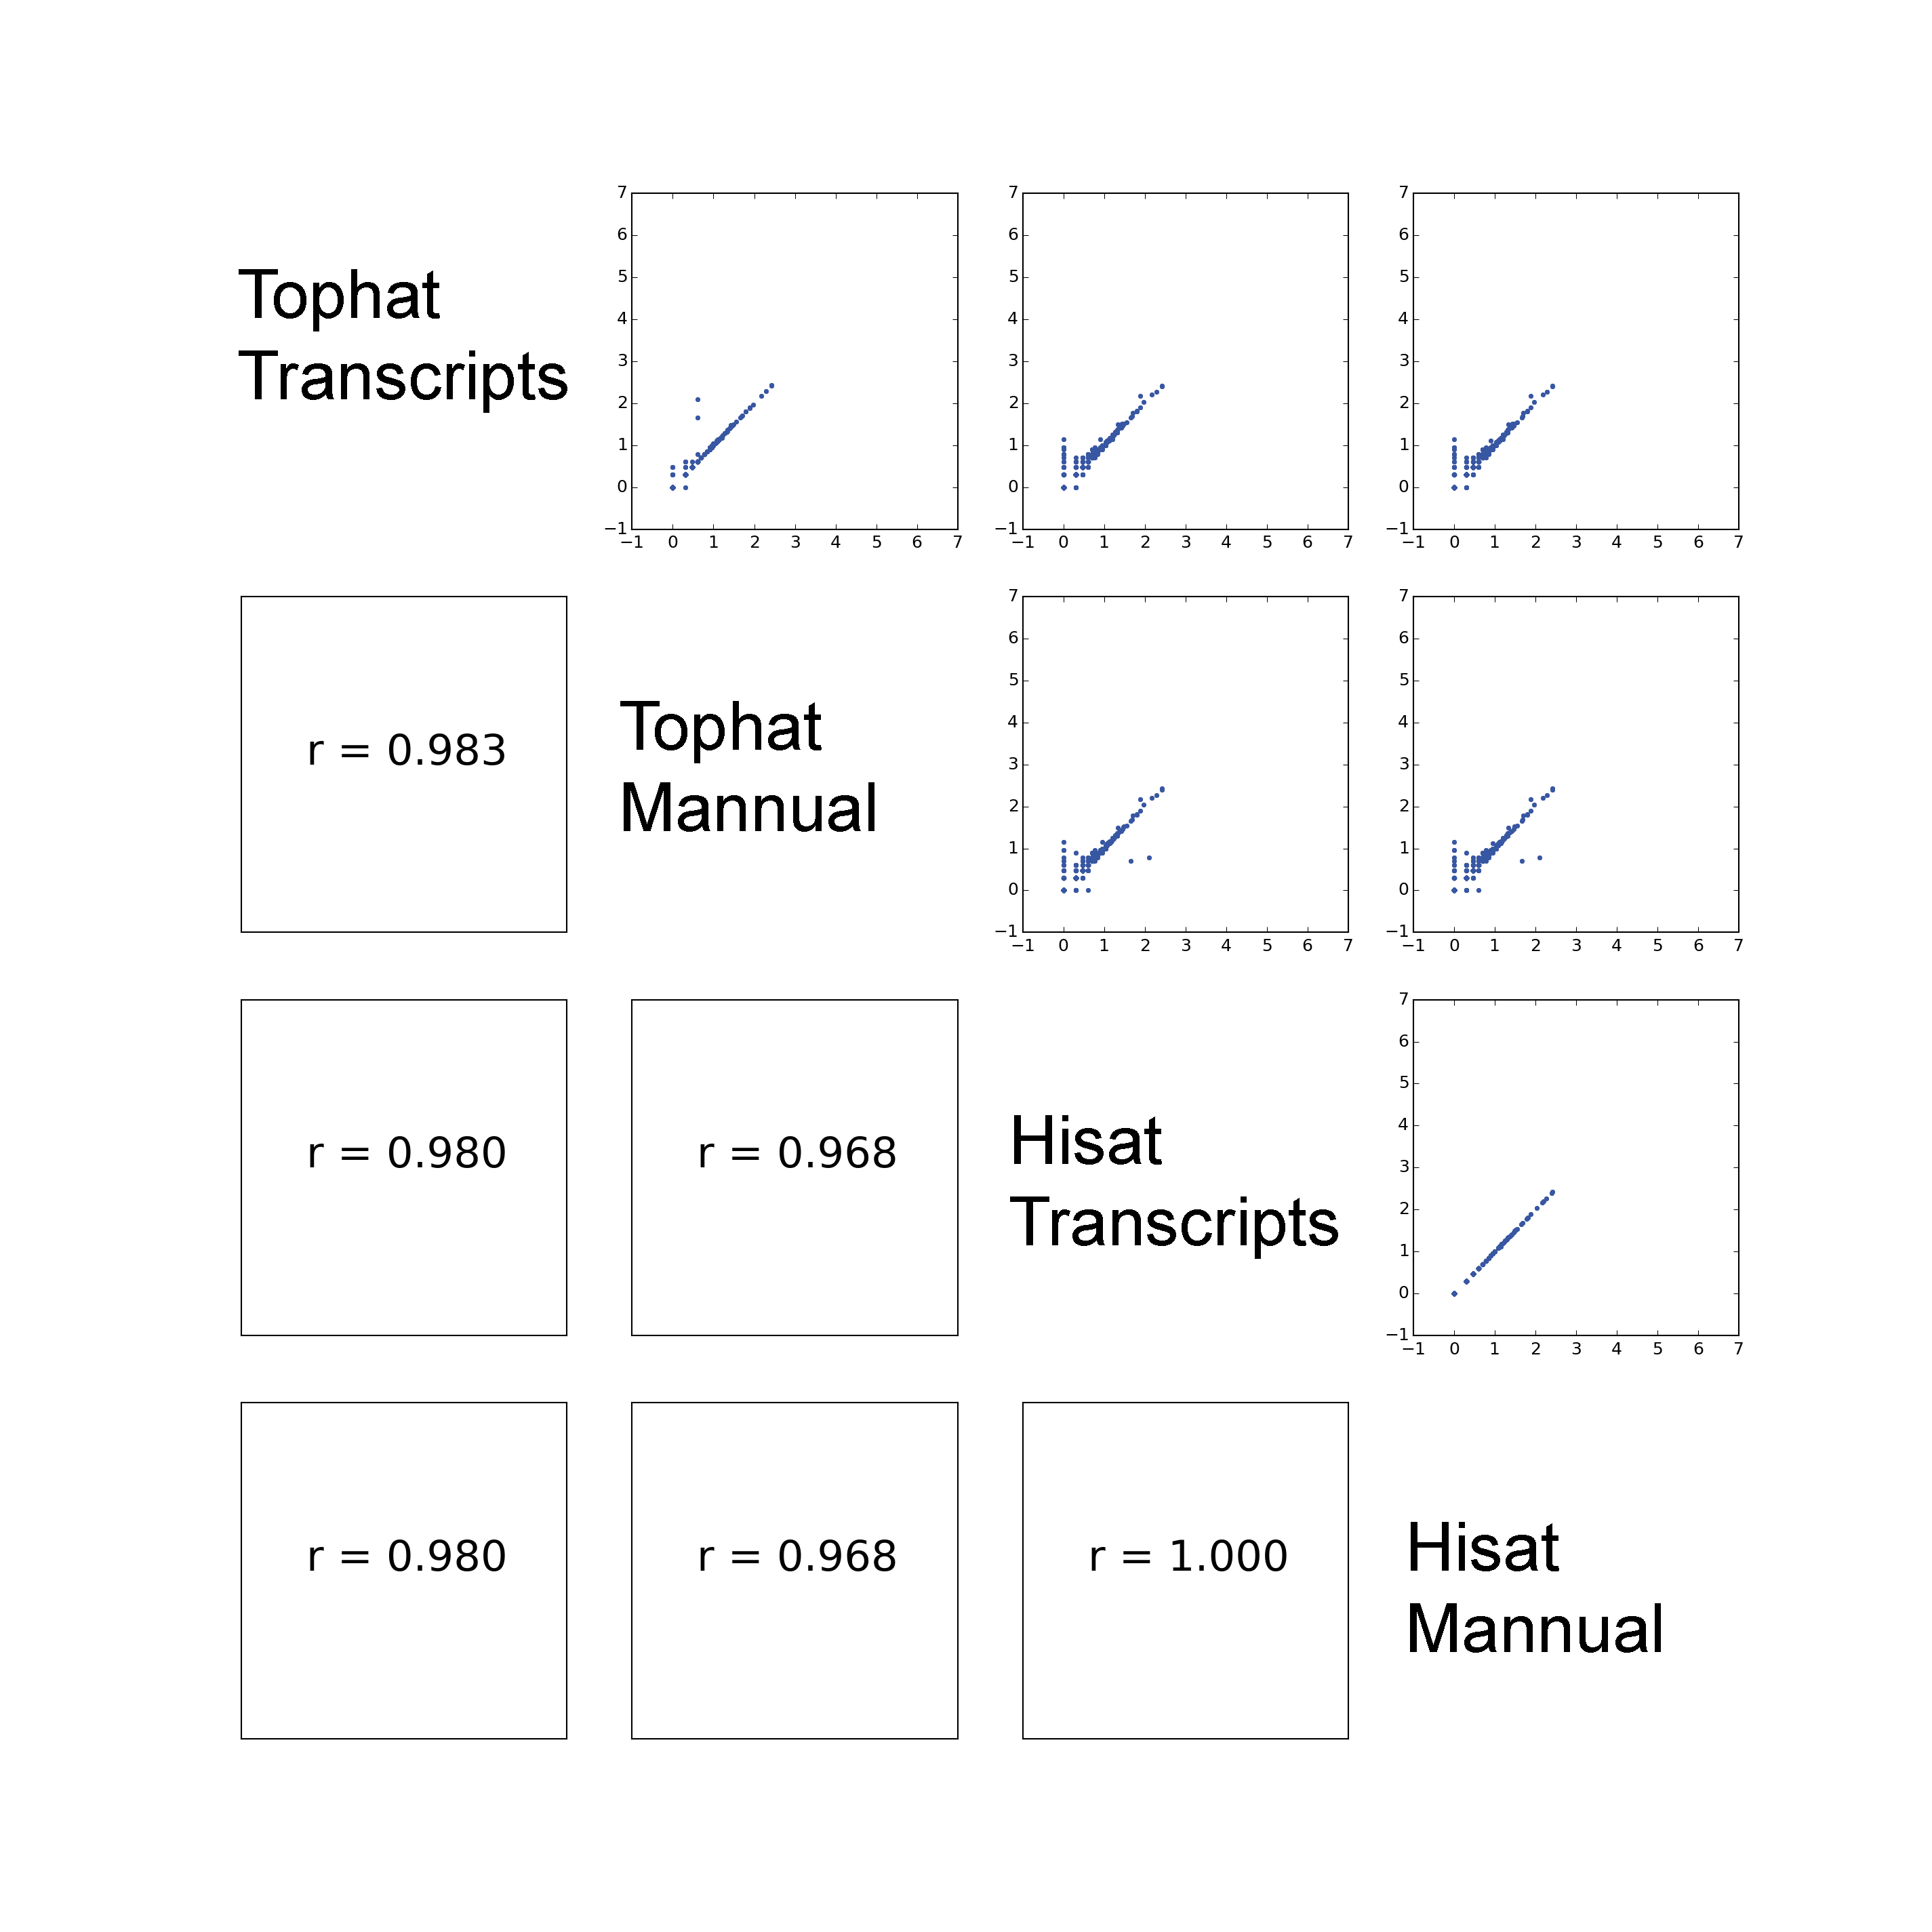
\includegraphics[height=3cm ]{NSMB_count}	 &
				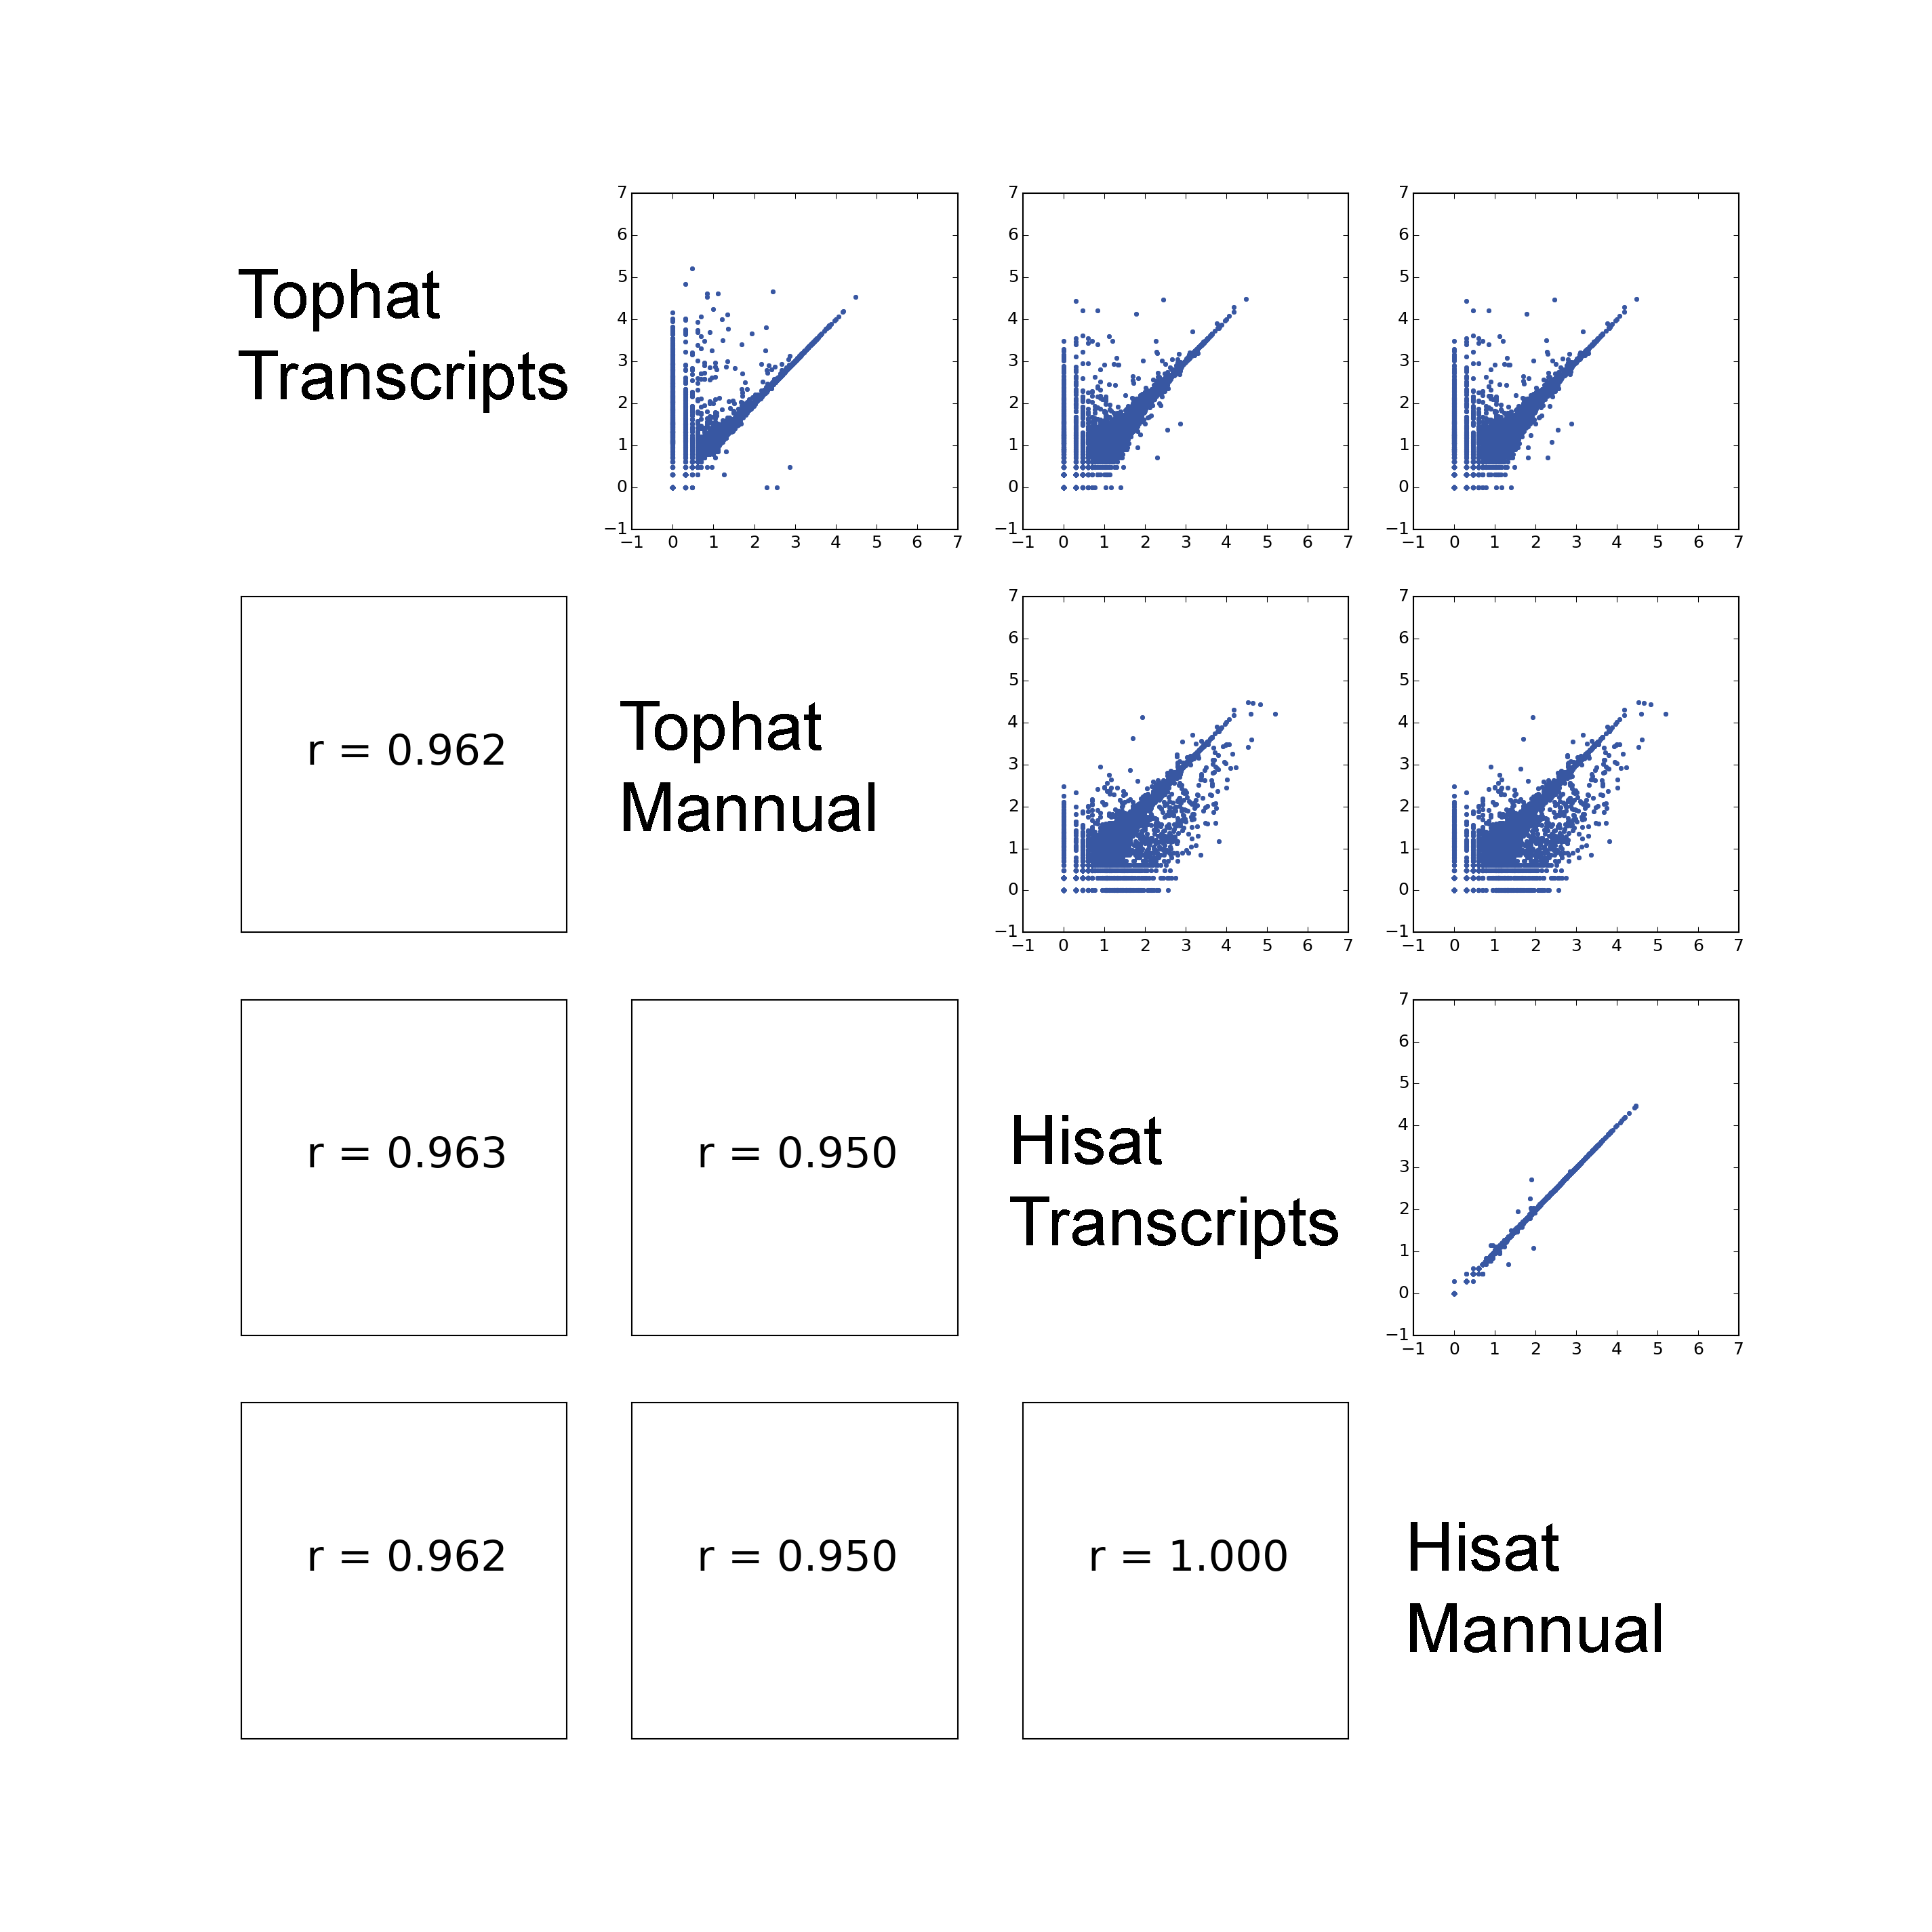
\includegraphics[height=3cm ]{Neo_count}	\\	
			\end{tabular}	
			\end{table}	
	\end{block}
\end{frame}



\subsection{3.Some case for different mapping.}

\begin{frame}[c,fragile]
	\frametitle{ Why some reads could only be mapped using Hisat. }
	\begin{block}{ case1. Hisat allows more mismatch.  }
		Tophat used \alert{"-N 2"} in the testing-script, which means the maxinum mismatch allowed in the given read. \\ \pause
		However, there were no such command for Hisat. \\ \pause
		If you require a maxinum mismatch for a successful mapping, just filter it by yourself using the resulting bam.
	\end{block}
\end{frame}

\begin{frame}[c,fragile]
	\begin{examples}
		$>$SRR534301.4\\
		\tiny{CGCCATCTGAGCCCTTCTCTTCAATCTCAGCCTTGAGGATCNNTAAGTCAGTAGTGAGCTCGTCCACCCGC\\TCCTNCNGNNCCTCCACCTCCTGCTGCAGG} \\
		\tiny{
			\begin{table}
			\centering
			\begin{tabular}{  C{1cm}  C{1.2cm}  C{1.2cm}  C{1.2cm}  C{1.2cm}  }
			\hline\noalign{\smallskip}
						& TT 	& HT  &	TM	 & HM  	\\
			\noalign{\smallskip}\hline\noalign{\smallskip}
			Chr:beg	&	-		& chr11:122928386   & - & chr11:122928386	\\
			Gene		&	-  	& HSPA8             & - & HSPA8          	\\
			\noalign{\smallskip}\hline 
			\end{tabular}
			\end{table}
		}
		\scriptsize{Tophat-Trans(TT) Hisat-Trans(HT) Tophat-Mannual(TM) Hisat2x-Mannual(HM).}
		\begin{lstlisting}[basicstyle=\tiny]
			
				SCORE START  END QSIZE IDENTITY CHRO STRAND  START    END      SPAN
				-------------------------------------------------------------------
				  94     1   101   101 100.0%     2   +   74597660  74597836    177
		
				00000063 tccacccgctcctncngnncctccacctcctgctgcagg 00000101
				>>>>>>>> ||||||||||||| | |  |||||||||||||||||||| >>>>>>>>
				74597798 tccacccgctccttcagtgcctccacctcctgctgcagg 74597836
		
		\end{lstlisting}
		\alert{3 mismatches}, above Tophat's cut-off(2).
		\end{examples}
	
\end{frame}

\begin{frame}[c,fragile]
	\frametitle{ Why some reads have different number of hits on genome. }
	\begin{block}{ case2. Pseudogenes.  }
		\begin{itemize}
			\item A read can both map to a protein-coding gene and a pseudogene. \\ \pause
			\item A junction for a protein-coding gene, and a mismatch for pseudogene. \\ \pause
			\item Junction is more realiable because of the existance of exons.	\\ \pause
			\item Penalty for mismatch is smaller.	\\ \pause
			\item Map reads to \alert{transcriptome first}.
		\end{itemize}
	\end{block}
\end{frame}

\begin{frame}[c,fragile]
	\begin{examples}
		$>$SRR534301.77\\
		\tiny{GTTGCTGGTGACAGCAAAAATGACCCACCAATGGAAGCAGCTGGCTTCACTGCTCAGGTGATTATCCTGAA\\CCATCCAGGCCAAATAAGCGCCGGCTATGC}
		\tiny{
			\begin{table}
			\centering
			\begin{tabular}{  C{1cm}  C{1.2cm}  C{1.2cm}  C{1.2cm}  C{1.2cm}  }
			\hline\noalign{\smallskip}
						& TT 	& HT  &	TM	 & HM  	\\
			\noalign{\smallskip}\hline\noalign{\smallskip}
			Chr:beg	&	chr6:74227944		& chr6:74227944 chr9:135895845    &	chr9:135895845 & chr6:74227944 chr9:135895845	\\
			Gene		&	EEF1A1            & \_\_too\_low\_aQual \_\_too\_low\_aQual &	\_\_no\_feature   & \_\_too\_low\_aQual \_\_too\_low\_aQual	\\
			\noalign{\smallskip}\hline
			\end{tabular}
			\end{table}
		}
		
		\scriptsize{Tophat-Trans(TT) Hisat-Trans(HT) Tophat-Mannual(TM) Hisat2x-Mannual(HM).}
		\begin{lstlisting}[basicstyle=\tiny]
			
				SCORE START  END QSIZE IDENTITY CHRO STRAND  START    END      SPAN
				-------------------------------------------------------------------
				101     1   101   101 100.0%     9   +  135895845 135895945    101
				100     1   101   101 100.0%     6   -   74227944  74228133    190

		\end{lstlisting}
		\end{examples}
	
\end{frame}

\begin{frame}[c,fragile]
	\frametitle{ Perfectly mapped on two sites, one protein-coding gene, one pseudo gene }
	\begin{examples}

		\begin{lstlisting}[basicstyle=\tiny]
			
				SCORE START  END QSIZE IDENTITY CHRO STRAND  START    END      SPAN
				-------------------------------------------------------------------
				101     1   101   101 100.0%     9   +  135895845 135895945    101
				100     1   101   101 100.0%     6   -   74227944  74228133    190
				
				chr6: EEF1A1, protein-coding gene with 90bp junction.
				00000051 tgctcag  == gtgattatcctgaaccatccaggccaaataagcgccggctatgc 00000101
				<<<<<<<< |||||||  == |||||||||||||||||||||||||||||||||||||||||||| <<<<<<<<
				74228083 tgctcag  == gtgattatcctgaaccatccaggccaaataagcgccggctatgc 74227944
				
				chr9: EEFAL3, pseudo gene with no junction.
				000000051 tgctcaggtgattatcctgaaccatccaggccaaataagcgccggctatg 000000100
				>>>>>>>>> |||||||||||||||||||||||||||||||||||||||||||||||||| >>>>>>>>>
				135895895 tgctcaggtgattatcctgaaccatccaggccaaataagcgccggctatg 135895944

		\end{lstlisting}
		\end{examples}
	
\end{frame}


\begin{frame}[c,fragile]
\frametitle{ Hisat reported a multiple hit while tophat thought it mapped uniquely to a protein coding gene. }
	\begin{examples}
		\tiny{
			\begin{table}
			\centering
			\begin{tabular}{  C{1cm}  C{1.2cm}  C{1.2cm}  C{1.2cm}  C{1.2cm}  }
			\hline\noalign{\smallskip}
						& TT 	& HT  &	TM	 & HM  	\\
			\noalign{\smallskip}\hline\noalign{\smallskip}
			Chr:beg	&	chr6:74227944		& chr6:74227944 chr9:135895845    &	chr9:135895845 & chr6:74227944 chr9:135895845	\\
			\noalign{\smallskip}\hline
			\end{tabular}
			\end{table}
		}
		\begin{lstlisting}[basicstyle=\tiny]
				chr6: EEF1A1, protein-coding gene with 90bp junction.
				00000051 tgctcag  == gtgattatcctgaaccatccaggccaaataagcgccggctatgc 00000101
				<<<<<<<< |||||||  == |||||||||||||||||||||||||||||||||||||||||||| <<<<<<<<
				74228083 tgctcag  == gtgattatcctgaaccatccaggccaaataagcgccggctatgc 74227944
				
				chr9: EEFAL3, pseudo gene with no junction.
				000000051 tgctcaggtgattatcctgaaccatccaggccaaataagcgccggctatg 000000100
				>>>>>>>>> |||||||||||||||||||||||||||||||||||||||||||||||||| >>>>>>>>>
				135895895 tgctcaggtgattatcctgaaccatccaggccaaataagcgccggctatg 135895944

		\end{lstlisting}
		\scriptsize{
			\begin{itemize}
				\item Transcripts-first mapping will consider protein-coding gene priorly. \\ \pause
				\item If not, it will consider pseudo gene priorly. \\ \pause
				\item Hisat reports all perfect-match sites.
			\end{itemize}
		}
		\end{examples}
	
\end{frame}

\subsection{4.Comparing with spike-in molecules.}

\begin{frame}[c,fragile]
	\frametitle{ Using relative total molecules. }
	\begin{block}{ ERCC spike-in detected. }
		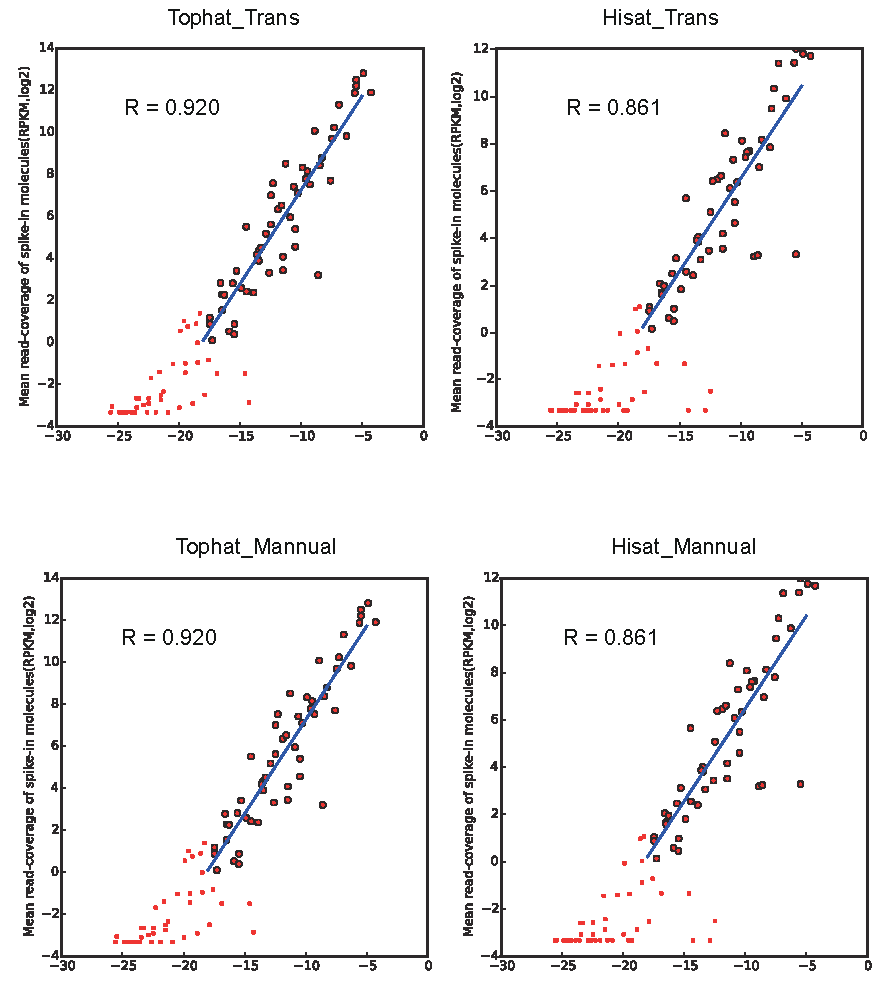
\includegraphics[height=5cm]{Ab_mol}
	\end{block}
\end{frame}

\subsection{5.Comparing with other methods.}
\begin{frame}[c,fragile]
	\frametitle{ Comparing RNA-seq with Taqman Gene Expression Assays. }
	\begin{block}{ Using method in nature07509, alternative isoform regulation in human tissue transcriptomes. }
		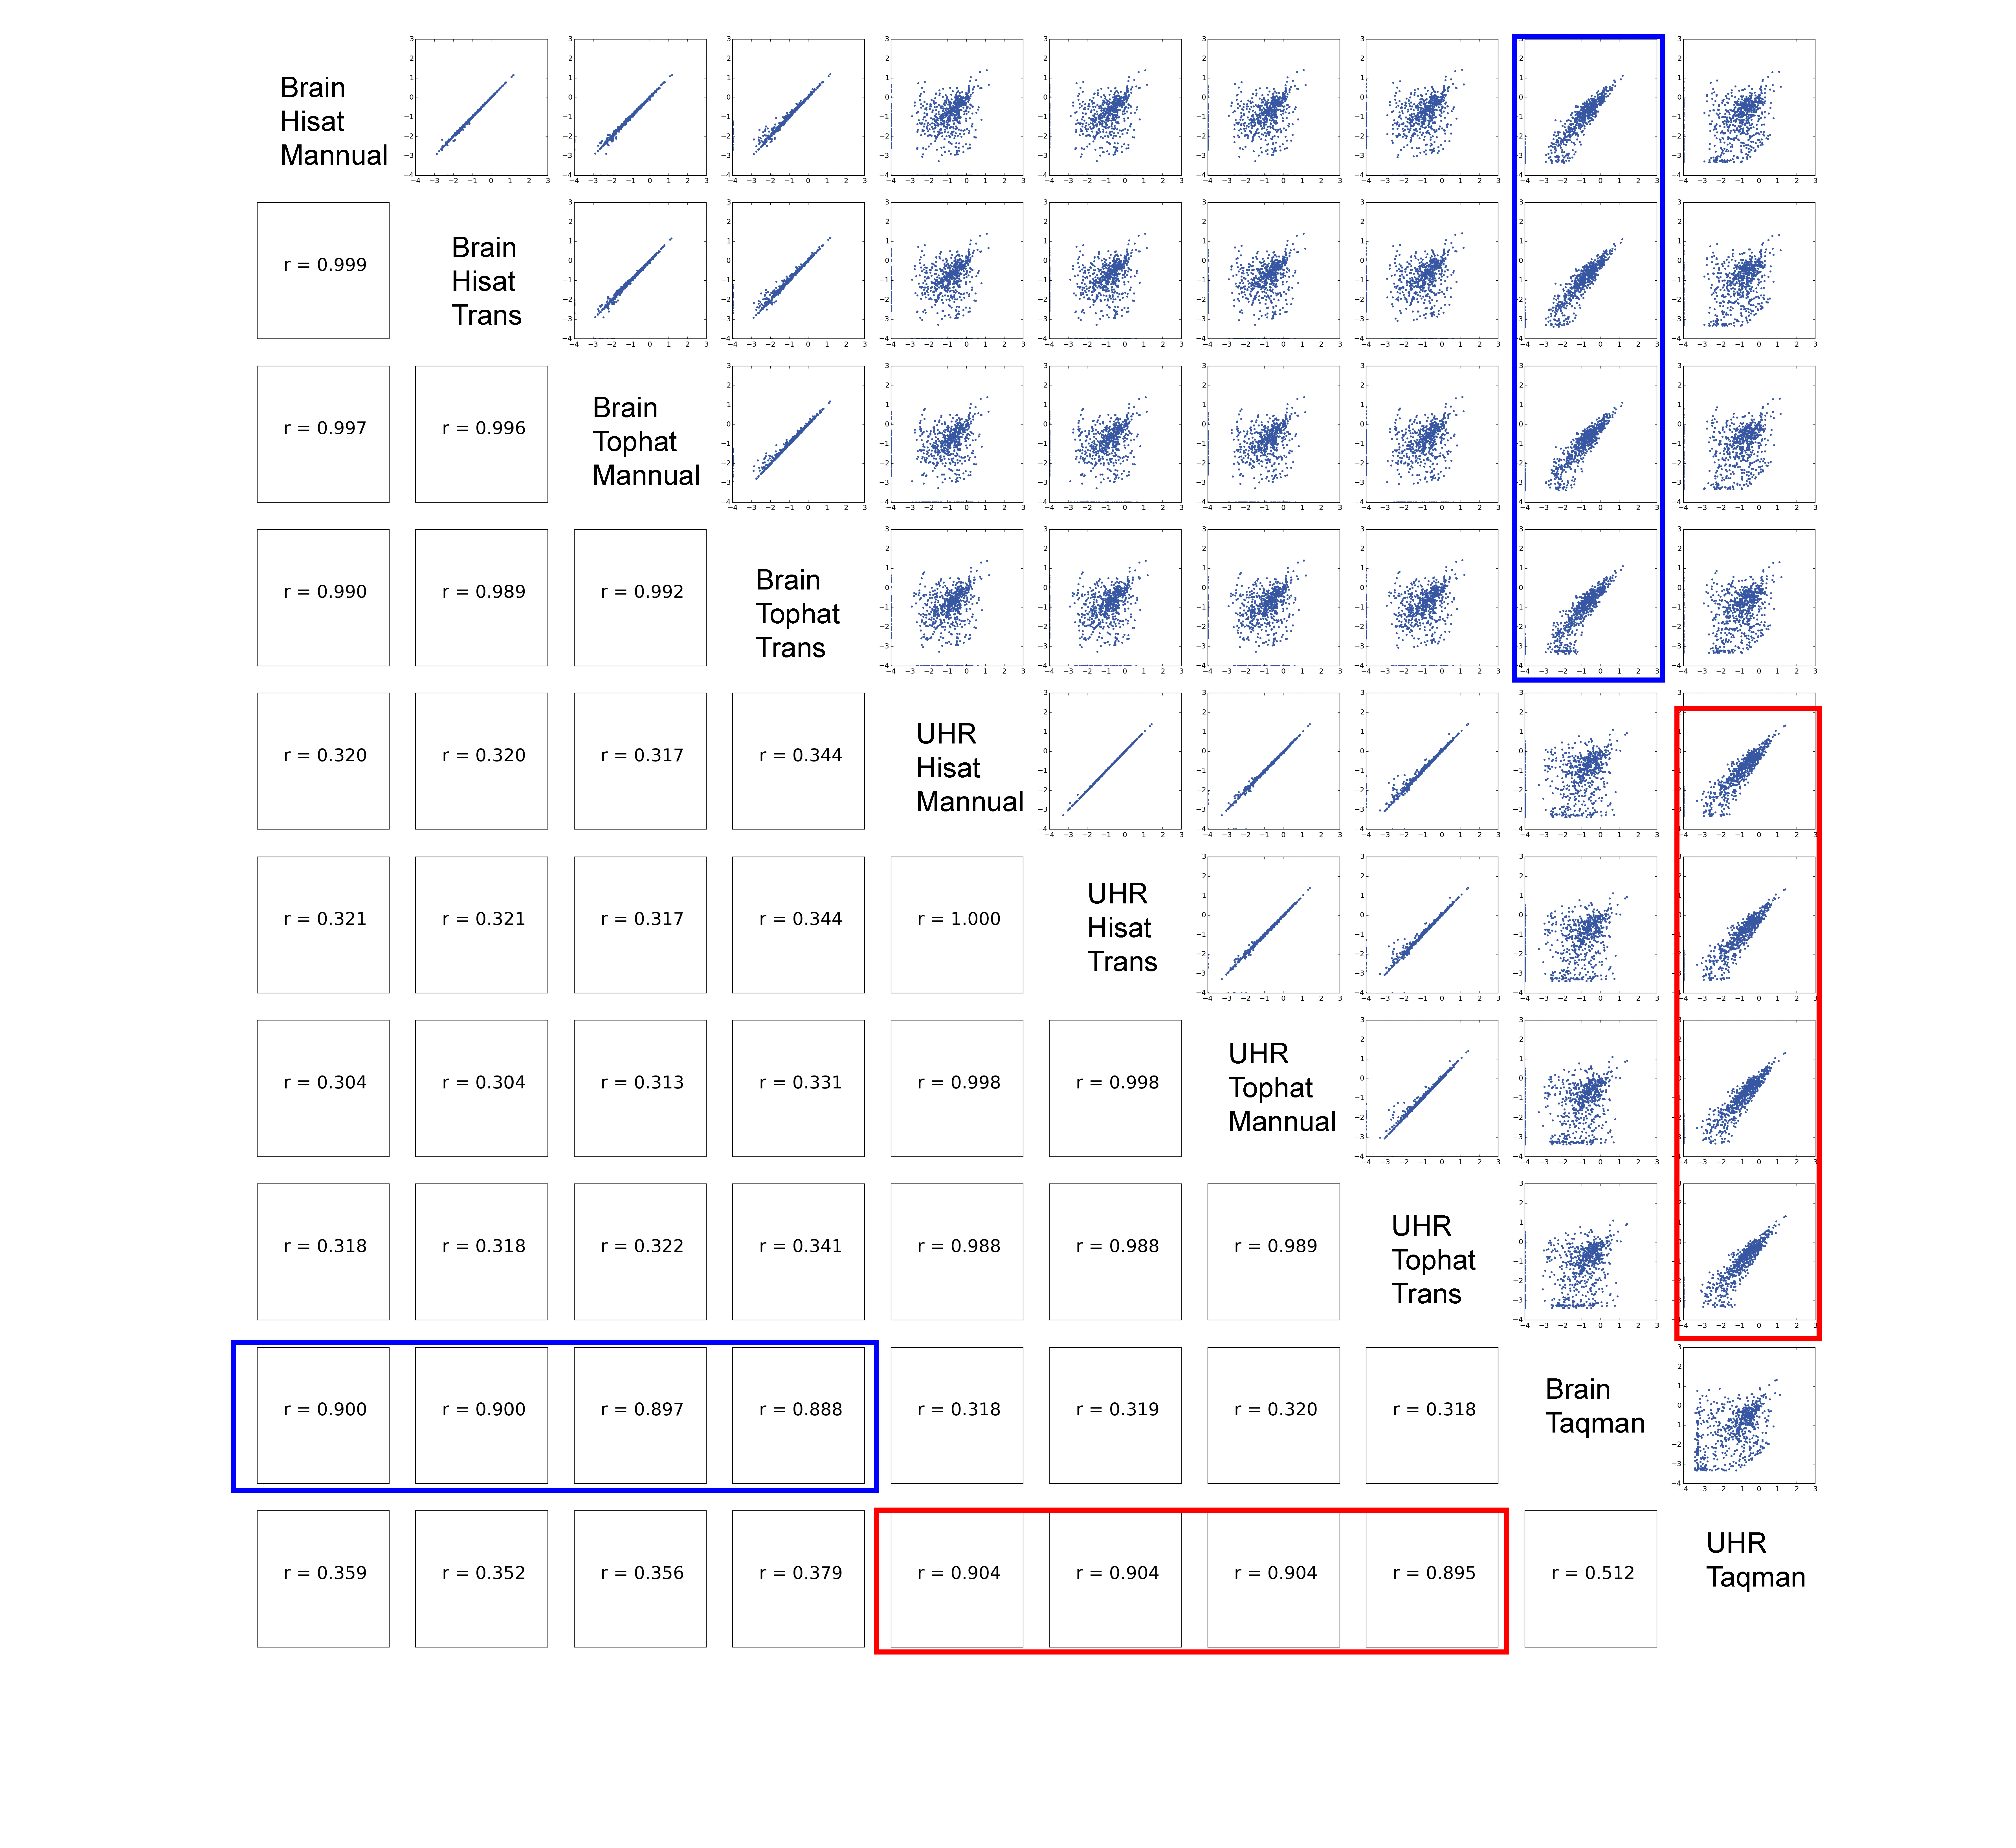
\includegraphics[height=5cm]{CompStandard}
	\end{block}
\end{frame}

\begin{frame}[c,fragile]
	\frametitle{ Comparing RNA-seq with Taqman Gene Expression Assays. }
	\begin{block}{ Result in nature07509. }
		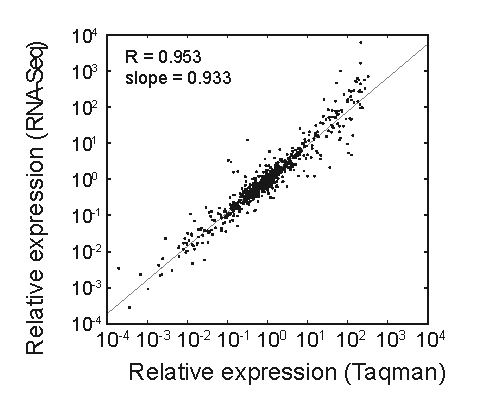
\includegraphics[height=5cm]{Standard_article}
	\end{block}
\end{frame}

\subsection{.}

\section{END}
\end{document}